
%% bare_conf.tex
%% V1.3
%% 2007/01/11
%% by Michael Shell
%% See:
%% http://www.michaelshell.org/
%% for current contact information.
%%
%% This is a skeleton file demonstrating the use of IEEEtran.cls
%% (requires IEEEtran.cls version 1.7 or later) with an IEEE conference paper.
%%
%% Support sites:
%% http://www.michaelshell.org/tex/ieeetran/
%% http://www.ctan.org/tex-archive/macros/latex/contrib/IEEEtran/
%% and
%% http://www.ieee.org/

%%*************************************************************************
%% Legal Notice:
%% This code is offered as-is without any warranty either expressed or
%% implied; without even the implied warranty of MERCHANTABILITY or
%% FITNESS FOR A PARTICULAR PURPOSE! 
%% User assumes all risk.
%% In no event shall IEEE or any contributor to this code be liable for
%% any damages or losses, including, but not limited to, incidental,
%% consequential, or any other damages, resulting from the use or misuse
%% of any information contained here.
%%
%% All comments are the opinions of their respective authors and are not
%% necessarily endorsed by the IEEE.
%%
%% This work is distributed under the LaTeX Project Public License (LPPL)
%% ( http://www.latex-project.org/ ) version 1.3, and may be freely used,
%% distributed and modified. A copy of the LPPL, version 1.3, is included
%% in the base LaTeX documentation of all distributions of LaTeX released
%% 2003/12/01 or later.
%% Retain all contribution notices and credits.
%% ** Modified files should be clearly indicated as such, including  **
%% ** renaming them and changing author support contact information. **
%%
%% File list of work: IEEEtran.cls, IEEEtran_HOWTO.pdf, bare_adv.tex,
%%                    bare_conf.tex, bare_jrnl.tex, bare_jrnl_compsoc.tex
%%*************************************************************************

% *** Authors should verify (and, if needed, correct) their LaTeX system  ***
% *** with the testflow diagnostic prior to trusting their LaTeX platform ***
% *** with production work. IEEE's font choices can trigger bugs that do  ***
% *** not appear when using other class files.                            ***
% The testflow support page is at:
% http://www.michaelshell.org/tex/testflow/



% Note that the a4paper option is mainly intended so that authors in
% countries using A4 can easily print to A4 and see how their papers will
% look in print - the typesetting of the document will not typically be
% affected with changes in paper size (but the bottom and side margins will).
% Use the testflow package mentioned above to verify correct handling of
% both paper sizes by the user's LaTeX system.
%
% Also note that the "draftcls" or "draftclsnofoot", not "draft", option
% should be used if it is desired that the figures are to be displayed in
% draft mode.
%
\documentclass[10pt, conference, letterpaper]{IEEEtran}

% Add the compsoc option for Computer Society conferences.
%
% If IEEEtran.cls has not been installed into the LaTeX system files,
% manually specify the path to it like:
% \documentclass[conference]{../sty/IEEEtran}


%\usepackage{fancyhdr}
%
\usepackage{tikzpagenodes}
\usepackage{epsfig}





% Some very useful LaTeX packages include:
% (uncomment the ones you want to load)


% *** MISC UTILITY PACKAGES ***
%
%\usepackage{ifpdf}
% Heiko Oberdiek's ifpdf.sty is very useful if you need conditional
% compilation based on whether the output is pdf or dvi.
% usage:
% \ifpdf
%   % pdf code
% \else
%   % dvi code
% \fi
% The latest version of ifpdf.sty can be obtained from:
% http://www.ctan.org/tex-archive/macros/latex/contrib/oberdiek/
% Also, note that IEEEtran.cls V1.7 and later provides a builtin
% \ifCLASSINFOpdf conditional that works the same way.
% When switching from latex to pdflatex and vice-versa, the compiler may
% have to be run twice to clear warning/error messages.






% *** CITATION PACKAGES ***
%
\usepackage{cite}
\usepackage{algorithm}
\usepackage{algorithmic}
% cite.sty was written by Donald Arseneau
% V1.6 and later of IEEEtran pre-defines the format of the cite.sty package
% \cite{} output to follow that of IEEE. Loading the cite package will
% result in citation numbers being automatically sorted and properly
% "compressed/ranged". e.g., [1], [9], [2], [7], [5], [6] without using
% cite.sty will become [1], [2], [5]--[7], [9] using cite.sty. cite.sty's
% \cite will automatically add leading space, if needed. Use cite.sty's
% noadjust option (cite.sty V3.8 and later) if you want to turn this off.
% cite.sty is already installed on most LaTeX systems. Be sure and use
% version 4.0 (2003-05-27) and later if using hyperref.sty. cite.sty does
% not currently provide for hyperlinked citations.
% The latest version can be obtained at:
% http://www.ctan.org/tex-archive/macros/latex/contrib/cite/
% The documentation is contained in the cite.sty file itself.






% *** GRAPHICS RELATED PACKAGES ***
%
\ifCLASSINFOpdf
  % \usepackage[pdftex]{graphicx}
  % declare the path(s) where your graphic files are
  % \graphicspath{{../pdf/}{../jpeg/}}
  % and their extensions so you won't have to specify these with
  % every instance of \includegraphics
  % \DeclareGraphicsExtensions{.pdf,.jpeg,.png}
\else
  % or other class option (dvipsone, dvipdf, if not using dvips). graphicx
  % will default to the driver specified in the system graphics.cfg if no
  % driver is specified.
  % \usepackage[dvips]{graphicx}
  % declare the path(s) where your graphic files are
  % \graphicspath{{../eps/}}
  % and their extensions so you won't have to specify these with
  % every instance of \includegraphics
  % \DeclareGraphicsExtensions{.eps}
\fi
% graphicx was written by David Carlisle and Sebastian Rahtz. It is
% required if you want graphics, photos, etc. graphicx.sty is already
% installed on most LaTeX systems. The latest version and documentation can
% be obtained at: 
% http://www.ctan.org/tex-archive/macros/latex/required/graphics/
% Another good source of documentation is "Using Imported Graphics in
% LaTeX2e" by Keith Reckdahl which can be found as epslatex.ps or
% epslatex.pdf at: http://www.ctan.org/tex-archive/info/
%
% latex, and pdflatex in dvi mode, support graphics in encapsulated
% postscript (.eps) format. pdflatex in pdf mode supports graphics
% in .pdf, .jpeg, .png and .mps (metapost) formats. Users should ensure
% that all non-photo figures use a vector format (.eps, .pdf, .mps) and
% not a bitmapped formats (.jpeg, .png). IEEE frowns on bitmapped formats
% which can result in "jaggedy"/blurry rendering of lines and letters as
% well as large increases in file sizes.
%
% You can find documentation about the pdfTeX application at:
% http://www.tug.org/applications/pdftex





% *** MATH PACKAGES ***
%
\usepackage[cmex10]{amsmath}
%\usepackage{amsthm}
% A popular package from the American Mathematical Society that provides
% many useful and powerful commands for dealing with mathematics. If using
% it, be sure to load this package with the cmex10 option to ensure that
% only type 1 fonts will utilized at all point sizes. Without this option,
% it is possible that some math symbols, particularly those within
% footnotes, will be rendered in bitmap form which will result in a
% document that can not be IEEE Xplore compliant!
%
% Also, note that the amsmath package sets \interdisplaylinepenalty to 10000
% thus preventing page breaks from occurring within multiline equations. Use:
%\interdisplaylinepenalty=2500
% after loading amsmath to restore such page breaks as IEEEtran.cls normally
% does. amsmath.sty is already installed on most LaTeX systems. The latest
% version and documentation can be obtained at:
% http://www.ctan.org/tex-archive/macros/latex/required/amslatex/math/

\usepackage{amssymb}



% *** SPECIALIZED LIST PACKAGES ***
%
%\usepackage{algorithmic}
% algorithmic.sty was written by Peter Williams and Rogerio Brito.
% This package provides an algorithmic environment fo describing algorithms.
% You can use the algorithmic environment in-text or within a figure
% environment to provide for a floating algorithm. Do NOT use the algorithm
% floating environment provided by algorithm.sty (by the same authors) or
% algorithm2e.sty (by Christophe Fiorio) as IEEE does not use dedicated
% algorithm float types and packages that provide these will not provide
% correct IEEE style captions. The latest version and documentation of
% algorithmic.sty can be obtained at:
% http://www.ctan.org/tex-archive/macros/latex/contrib/algorithms/
% There is also a support site at:
% http://algorithms.berlios.de/index.html
% Also of interest may be the (relatively newer and more customizable)
% algorithmicx.sty package by Szasz Janos:
% http://www.ctan.org/tex-archive/macros/latex/contrib/algorithmicx/




% *** ALIGNMENT PACKAGES ***
%
%\usepackage{array}
% Frank Mittelbach's and David Carlisle's array.sty patches and improves
% the standard LaTeX2e array and tabular environments to provide better
% appearance and additional user controls. As the default LaTeX2e table
% generation code is lacking to the point of almost being broken with
% respect to the quality of the end results, all users are strongly
% advised to use an enhanced (at the very least that provided by array.sty)
% set of table tools. array.sty is already installed on most systems. The
% latest version and documentation can be obtained at:
% http://www.ctan.org/tex-archive/macros/latex/required/tools/

\usepackage{color}

\usepackage{mdwmath}
\usepackage{mdwtab}
% Also highly recommended is Mark Wooding's extremely powerful MDW tools,
% especially mdwmath.sty and mdwtab.sty which are used to format equations
% and tables, respectively. The MDWtools set is already installed on most
% LaTeX systems. The lastest version and documentation is available at:
% http://www.ctan.org/tex-archive/macros/latex/contrib/mdwtools/


% IEEEtran contains the IEEEeqnarray family of commands that can be used to
% generate multiline equations as well as matrices, tables, etc., of high
% quality.


%\usepackage{eqparbox}
% Also of notable interest is Scott Pakin's eqparbox package for creating
% (automatically sized) equal width boxes - aka "natural width parboxes".
% Available at:
% http://www.ctan.org/tex-archive/macros/latex/contrib/eqparbox/





% *** SUBFIGURE PACKAGES ***
%\usepackage[tight,footnotesize]{subfigure}
% subfigure.sty was written by Steven Douglas Cochran. This package makes it
% easy to put subfigures in your figures. e.g., "Figure 1a and 1b". For IEEE
% work, it is a good idea to load it with the tight package option to reduce
% the amount of white space around the subfigures. subfigure.sty is already
% installed on most LaTeX systems. The latest version and documentation can
% be obtained at:
% http://www.ctan.org/tex-archive/obsolete/macros/latex/contrib/subfigure/
% subfigure.sty has been superceeded by subfig.sty.



%\usepackage[caption=false]{caption}
%\usepackage[font=footnotesize]{subfig}
% subfig.sty, also written by Steven Douglas Cochran, is the modern
% replacement for subfigure.sty. However, subfig.sty requires and
% automatically loads Axel Sommerfeldt's caption.sty which will override
% IEEEtran.cls handling of captions and this will result in nonIEEE style
% figure/table captions. To prevent this problem, be sure and preload
% caption.sty with its "caption=false" package option. This is will preserve
% IEEEtran.cls handing of captions. Version 1.3 (2005/06/28) and later 
% (recommended due to many improvements over 1.2) of subfig.sty supports
% the caption=false option directly:
%\usepackage[caption=false,font=footnotesize]{subfig}
%
% The latest version and documentation can be obtained at:
% http://www.ctan.org/tex-archive/macros/latex/contrib/subfig/
% The latest version and documentation of caption.sty can be obtained at:
% http://www.ctan.org/tex-archive/macros/latex/contrib/caption/




% *** FLOAT PACKAGES ***
%
%\usepackage{fixltx2e}
% fixltx2e, the successor to the earlier fix2col.sty, was written by
% Frank Mittelbach and David Carlisle. This package corrects a few problems
% in the LaTeX2e kernel, the most notable of which is that in current
% LaTeX2e releases, the ordering of single and double column floats is not
% guaranteed to be preserved. Thus, an unpatched LaTeX2e can allow a
% single column figure to be placed prior to an earlier double column
% figure. The latest version and documentation can be found at:
% http://www.ctan.org/tex-archive/macros/latex/base/



%\usepackage{stfloats}
% stfloats.sty was written by Sigitas Tolusis. This package gives LaTeX2e
% the ability to do double column floats at the bottom of the page as well
% as the top. (e.g., "\begin{figure*}[!b]" is not normally possible in
% LaTeX2e). It also provides a command:
%\fnbelowfloat
% to enable the placement of footnotes below bottom floats (the standard
% LaTeX2e kernel puts them above bottom floats). This is an invasive package
% which rewrites many portions of the LaTeX2e float routines. It may not work
% with other packages that modify the LaTeX2e float routines. The latest
% version and documentation can be obtained at:
% http://www.ctan.org/tex-archive/macros/latex/contrib/sttools/
% Documentation is contained in the stfloats.sty comments as well as in the
% presfull.pdf file. Do not use the stfloats baselinefloat ability as IEEE
% does not allow \baselineskip to stretch. Authors submitting work to the
% IEEE should note that IEEE rarely uses double column equations and
% that authors should try to avoid such use. Do not be tempted to use the
% cuted.sty or midfloat.sty packages (also by Sigitas Tolusis) as IEEE does
% not format its papers in such ways.





% *** PDF, URL AND HYPERLINK PACKAGES ***
%
%\usepackage{url}
% url.sty was written by Donald Arseneau. It provides better support for
% handling and breaking URLs. url.sty is already installed on most LaTeX
% systems. The latest version can be obtained at:
% http://www.ctan.org/tex-archive/macros/latex/contrib/misc/
% Read the url.sty source comments for usage information. Basically,
% \url{my_url_here}.





% *** Do not adjust lengths that control margins, column widths, etc. ***
% *** Do not use packages that alter fonts (such as pslatex).         ***
% There should be no need to do such things with IEEEtran.cls V1.6 and later.
% (Unless specifically asked to do so by the journal or conference you plan
% to submit to, of course. )


% correct bad hyphenation here
%\hyphenation{op-tical net-works semi-conduc-tor}
%
%\fancyhf{}
%\pagestyle{fancy}
%\fancyhead[C]{\small 2015 International Conference on Indoor Positioning and Indoor Navigation (IPIN), 13-16 October 2015, Banff, Alberta, Canada} 
%\pagenumbering{gobble}
%\renewcommand{\headrulewidth}{0pt}
%\renewcommand{\footrulewidth}{0pt}
\newtheorem{definition}{Definition}
\newtheorem{theorem}{Theorem}
\newtheorem{proof}{Proof}
\newtheorem{lemma}{Lemma}
\newtheorem{assumption}{Assumption}
\newtheorem{proposition}{Proposition}
\newtheorem{example}{Example}
\newtheorem{problem}{Problem}

\renewcommand\floatpagefraction{.9}
\renewcommand\topfraction{.9}
\renewcommand\bottomfraction{.9}
\renewcommand\textfraction{.1}
\setcounter{totalnumber}{50}
\setcounter{topnumber}{50}
\setcounter{bottomnumber}{50}

\setlength{\floatsep} {5pt plus 3pt minus 1pt}
\setlength{\textfloatsep} {5pt plus 3pt minus 1pt}

%\renewcommand{\baselinestretch}{1.1}
\begin{document}



%
% paper title
% can use linebreaks \\ within to get better formatting as desired
\title{WarpMap: Accurate and Efficient Indoor Location by Dynamic Warping in Sequence-Type Radio-map}


% author names and affiliations
% use a multiple column layout for up to three different
% affiliations
\author{
\IEEEauthorblockN{Xuehan Ye, Yongcai Wang}
\IEEEauthorblockA{CS, 
Renmin University\\
Beijing China\\
ycw@ruc.edu.cn}
\and
\IEEEauthorblockN{Wei Hu, Lei Song}
\IEEEauthorblockA{IIIS,
Tsinghua University\\
Beijing, China\\
huwei12@mails.tsinghua.edu.cn\\
leisong03@gmail.com}
\and
\IEEEauthorblockN{Deying Li}
\IEEEauthorblockA{
Renmin University\\
Beijing, China\\
deyingli@ruc.edu.cn}
\and
}

% conference papers do not typically use \thanks and this command
% is locked out in conference mode. If really needed, such as for
% the acknowledgment of grants, issue a \IEEEoverridecommandlockouts
% after \documentclass

% for over three affiliations, or if they all won't fit within the width
% of the page, use this alternative format:
% 
%\author{\IEEEauthorblockN{Michael Shell\IEEEauthorrefmark{1},
%Homer Simpson\IEEEauthorrefmark{2},
%James Kirk\IEEEauthorrefmark{3}, 
%Montgomery Scott\IEEEauthorrefmark{3} and
%Eldon Tyrell\IEEEauthorrefmark{4}}
%\IEEEauthorblockA{\IEEEauthorrefmark{1}School of Electrical and Computer Engineering\\
%Georgia Institute of Technology,
%Atlanta, Georgia 30332--0250\\ Email: see http://www.michaelshell.org/contact.html}
%\IEEEauthorblockA{\IEEEauthorrefmark{2}Twentieth Century Fox, Springfield, USA\\
%Email: homer@thesimpsons.com}
%\IEEEauthorblockA{\IEEEauthorrefmark{3}Starfleet Academy, San Francisco, California 96678-2391\\
%Telephone: (800) 555--1212, Fax: (888) 555--1212}
%\IEEEauthorblockA{\IEEEauthorrefmark{4}Tyrell Inc., 123 Replicant Street, Los Angeles, California 90210--4321}}
%
%\author{
%\IEEEauthorblockN{Xuehan Ye\IEEEauthorrefmark{1}, Wei Hu\IEEEauthorrefmark{2}, Yongcai Wang\IEEEauthorrefmark{3}, Lei Song \IEEEauthorrefmark{2}, Deying Li
%\IEEEauthorrefmark{3}}
%\IEEEauthorblockA{\IEEEauthorrefmark{1}Department of Computer Science, Beijing Forest University, Beijing, China}
%\IEEEauthorblockA{\IEEEauthorrefmark{1}Institute for Interdisciplinary Information Sciences, Tsinghua University, Beijing, China}
%\IEEEauthorblockA{\IEEEauthorrefmark{1}Department of computer sciences, Renmin University, Beijing, China\\
%Email: wangyc@tsinghua.edu.cn}
%}




% use for special paper notices
%\IEEEspecialpapernotice{(Invited Paper)}




% make the title area
\maketitle

%\begin{tikzpicture}[remember picture,overlay]
%    \node[align=center] at ([yshift=2em] current page text area.north) {\small 2015 International Conference on Indoor Positioning and Indoor Navigation (IPIN), 13-16 October 2015, Banff, Alberta, Canada};
   % \node[align=center,text=blue] at ([yshift=-1em]current page text area.south) {This is some
    %        footer text};
%  \end{tikzpicture}%
%\renewcommand{\baselinestretch}{1.09}
\begin{abstract}
%\boldmath
Radio-map based method has been widely used for indoor location and navigation, 
%due to its advantage of characterizing a location by radio signal strength (RSS) signature captured at the location, which maps the signal space to physical space to tame the indoor radio propagation dynamics. However, long existing 
but remained challenges are: 1) laborious efforts to calibrate a fine-grained radio-map, and 2) the locating result inaccuracy and not robust problems due to random RSS noises. An efficient way to overcome these problems is to collect RSS signatures along indoor paths and utilize sequence matching to enhance the location robustness. But, due to problems of indoor path combinational explosion, random RSS loss during movement,  and moving speed disparity during online and offline phases, how to exploit sequence matching in radio-map remains difficult. 


%Existing works on radio-map indoor location methods devoted deliberated efforts to utilize additional information such as inertial data, path constraint, and motion continuity of targets to reduce the radio-map calibration cost and to enhance the location accuracy. 
%for reducing the calibration cost by utilizing additional inertial and map information; and enhanced the location accuracy by using additional motion constraints and map constraint information using Bayesian filter or Markov random field etc, 
%however the radio-map itself has been rarely revised. %without modifying the the radio-map itself. 
	This paper proposes WarpMap,  an accurate and efficient indoor location method by dynamic warping in sequence-type radio-map. Its distinct features include 1) an undirected graph model (tracegraph) for storing smoothed RSS sequence in a sequence-type radio-map; and 2) a sub-sequence dynamic time warping (SDTW) algorithm for on-line locating. In particular, in trace-graph, each vertex represents a RSS sequence of a indoor path segment. The graph is constructed off-line by trimming and filtering the noisy RSS sequences collected by user via traversing the indoor paths once. It embeds the path constraint and motion continuity information directly into the radio-map model,  while overcoming the indoor path combinational explosion problem. Based on the trace-graph, a subsequence dynamic time warping algorithm (SDTW) for on-line locating was proposed. It includes steps of i) candidate sequence set extraction; ii) warping distance calculation; and iii) location determination by the end-point of the best matched sub-sequence. Sequence warping can tolerate  random RSS disparities at discrete points and and can also handle the moving speed differences in on-line and off-line phases. The impacts of different warping distance functions, RSS preprocessing techniques, and fusion extensions were investigated.  
%because the dynamic sequence warping algorithm conducts online locating via sequence matching, which can tolerate the random RSS disparities at discrete points and random noises much better than the traditional point matching. 
%We further proposed detailed data clean and preprocessing methods to address practical issues including the MAC ambiguity, RSS loss and device disparity etc. 
%In open area, where paths are hard to specify, WarpMap is reduced a graph in which each node has full connection to its neighbors. We can still utilize the idea of sequence matching to enhance locating accuracy. 
Property analysis and extensive  experiments in office environments verified the efficiency and accuracy of WarpMap. It can be calibrated within several minutes for $1000 m^2$ area; provides robust and accurate locating in different settings, and overall nearly 20\% accuracy improvements than the state-of-the-art radio-map  method.  
\end{abstract}
% IEEEtran.cls defaults to using nonbold math in the Abstract.
% This preserves the distinction between vectors and scalars. However,
% if the conference you are submitting to favors bold math in the abstract,
% then you can use LaTeX's standard command \boldmath at the very start
% of the abstract to achieve this. Many IEEE journals/conferences frown on
% math in the abstract anyway.

% no keywords

%\begin{keywords}

%\end{keywords}


% For peer review papers, you can put extra information on the cover
% page as needed:
% \ifCLASSOPTIONpeerreview
% \begin{center} \bfseries EDICS Category: 3-BBND \end{center}
% \fi
%
% For peerreview papers, this IEEEtran command inserts a page break and
% creates the second title. It will be ignored for other modes.
\IEEEpeerreviewmaketitle

\section{Introduction}

Radio-map locating method, which characterizes each location-of-interest by the radio signal strength (RSS) signature, has attracted great attentions for indoor positioning and navigation. It maps the signal space to physical space to tame the indoor radio propagation dynamics; becomes popular nowadays for the broad availability of WiFi coverage and free-of-charge of radio RSS measurement. Comparing to other locating techniques, it provides key advantages including: 1) purely software-implementable on mobile phones without requiring additional hardware infrastructure; 2) privacy protection for working in navigation mode; and 3) reasonable accuracy  with errors around 2-3 meters \cite{bahl_radar:_2000, haque_profiling-based_2013}. %To determine the position of a wireless device, 

More specifically, routine of radio-map method generally has an offline site survey and an online locating phases. The offline site survey is to calibrate the received signal strengths (RSS) at different known locations, which builds a \emph{radio-map}. The RSS signatures at a location can be modeled by mean value, or probabilistic density function of received RSS values, which form deterministic \cite{bahl_radar:_2000}\cite{haque_profiling-based_2013} or probabilistic-type \cite{Youssef:2005:HWL:1067170.1067193}\cite{King:2006:CPI:1160987.1160995}  radio-map respectively.  In the online phase, a mobile target captures on-site RSS and searches in the radio-map, to find the location whose RSS signature best matches the measured RSS to determine the real-time location of the target. 

%Location fingerprinting consists of an offline training phase and an online position determination phase. In the offline phase, RSS values at different known locations are collected and saved in a \emph{radio map}.
%In the online phase, the RSS values are measured by a device, and its location is determined by comparing these RSS values to the ones in the radio map.

%Despite its wide applicability in applications, location fingerprinting has two major drawbacks:
%(i) It is very laborious to build the radio map. The RSS values at many locations need to be measured, and these locations need to be recorded manually. To reduce noise, at the same position the RSS values are usually measured multiple times.
%(ii) Location fingerprinting usually has limited accuracy, since the relation between RSS and location is very complicated -- RSS is intrinsically random, and the RSS measured at the same position are affected by many factors such as the orientation of the measuring device. The localization accuracy is therefore not always reliable.

Despite of the advantages, several practical issues must be considered for practical applications: (i) it is very laborious to calibrate a fine-grained radio-map point-by-point, especially for large application areas;  
(ii) the point-type matching at discrete times and locations is sensitive to random online RSS noises and environment dynamics. 
To overcome these problems, previous work have devoted deliberated efforts to exploit different kinds of information and methods to reduce radio-map calibration cost and to improve the positioning accuracy and robustness. 

A major approach to reduce calibration cost is unsupervised indoor locating method\cite{}, which exploited environment signature including magnetic fluctuation, illumination intensity at specific spots as internal landmarks\cite{}, and used dead reckoning by mobile phones\cite{} to track the inertial landmarks to conduct locating, so as to avoid the manually radio-map calibration. %Such methods tried to avoid the offline calibration cost, whereas, need many additional sensors and higher computation cost to discover the internal landmarks and to associate them to locations. 
Another major approach exploited automatic labeling \cite{}\cite{}, which leveraged dead reckoning by motion sensors to construct a radio-map firstly in the radio space, then stretch and associate the radio-space geometry to physical space by geometrical matching using the path information  from the floor-plan.  Other approaches also exploited Expectation-Maximisation (EM) and Manifold methods to learn radio-map parameters by training  parametric radio-map models\cite{}\cite{}. These methods, however, generally require additional sensors or depend heavily on the accuracy of dead reckoning, which is known difficult by using commodity mobile phones \cite{}\cite{}. The inaccuracy of radio-map model may also degrade the performance of locating accuracy.  
    
In the other aspect, for improving the locating accuracy and robustness, a major approach is to build fine-grained or probabilistic radio-map to preserve more information \cite{}\cite{} in the radio-map, but such kind methods requires higher calibration cost.  Another major approach is to exploit Support Vector Machine (SVM) or $K$-Nearest Neighbor algorithms etc to tolerate random noises in the locating process \cite{}\cite{}. Other approaches used information fusion techniques, which exploited the motion continuity information, floor map information to design Bayesian filter\cite{}, particle filter\cite{}, Hidden Markov Model\cite{}, and Markov Random Field models \cite{} to narrow down the search space,  and posteriorly improve the locating accuracy against noises. These methods depend on information fusion technique to utilize the motion constraint and the path constraint, for these information are not properly contained in the point-type radio-map model. 

A more direct and promising way to ease the radio-map calibration and to improve the location robustness as well is to collect RSS sequence along indoor paths to build sequence-type radio-map, and to exploit the motion constraint and path constraint embedded in the sequential RSS signatures to improve the positioning accuracy. But, several practical difficulties have obstructed such a direct approach: 1) the number of indoor paths grow exponentially with the number of path segments, making storage of RSS sequences for all paths inaccessible. Note that a path segment is the path within two adjacent crosses. 2) The random missing of RSS measurements during user movement, causing disparity of RSS sequence signatures in online phase and offline phase. 3) The moving speeds and moving patterns of users in online phase and offline phase maybe different, leading to difficulty of accurate sequence matching. As a result, although some practical works collect RSS sequences along paths\cite{}, the collected sequences are divided into points to construct point-type radio-map. The path structure and motion constraints are lost in the radio-map, which is however compensated by post-processing via information fusion, such as map-matching and particle filter using additional information\cite{}.





%which can potentially enhance the location accuracy is not efficiently modeled in the point-type radio-map; (iii) the motion continuity and path constraint are not efficiently utilized in the online locating routine. As a result, previous studies need to devote deliberated efforts to reduce radio-map calibration \cite{}\cite{} cost by exploiting additional information including internal sensor data and floor map information; Motion continuity and floor map constraints are utilized only in post processing process to enhance locating accuracy using Bayesian rules \cite{} and Markov Random Field models\cite{}.  


%Motivated by the above disadvantages, we propose a novel location fingerprinting framework based on sequence, which is referred to as \emph{sequence-type} location fingerprinting, as opposed to the original \emph{point-type} method. The idea behind our method is to use sequences of RSS values measured along different routes, instead of RSS values at separate points. The radio map is a collection of sequences, each of which contains RSS values measured along a route whose location is known. In the online plase, a sequence of RSS values are measured along a short route. Then dynamic time warping (DTW) is used to find an optimal alignment between this RSS sequence and a subsequence in the radio map, which will give an estimate of the location of the route.

This paper revisits sequence matching in radio-map. It proposes \emph{WarpMap} to tackle the sequence radio-map construction and online matching challenges. 
The key idea is to model the RSS sequence signatures of indoor path by an undirected \emph{tracegraph} model. Each vertex in the graph models the RSS sequence of a path segment. By such a method, the tracegraph can be  trained by user traversing the indoor paths once  by capturing RSS signatures during movement. The random RSS missing problem is addressed by a collaborative filtering method, which on one hand smooths the measured RSS values, on the other hand complements the missing values. Based on the tracegraph, RSS sequence for each selected path can be easily generated. 
Then, a sub-sequence dynamic time warping (SDTW) algorithm is proposed to conduct sequence matching in online phase. It finds the best match from the RSS sequence measured online in a short moving window to a subsequence in the tracegraph. It tolerates the moving speed differences by warping \cite{} instead of one-to-one matching. It includes a candidate sequence set extraction step and a location determination phase, which will be detailed in Section III. More specifically, our contributions include:
\begin{enumerate}
\item A WarpMap model represented by undirected graph $G=(V,E)$, where $V$ represents 
RSS signatures on path segments and $E$ represents adjacency of  path segments.  
\item A fast calibration process to build $G$ by user traversing indoor routes for once, and a collaborative filtering method to smooth the noisy RSS data. 
\item In online phase, a potential path extraction algorithm to extract from $G$ the potential paths that the target maybe undergoing, based on the list of real-time detected APs. It prepares a small \emph{candidate sequence set (CSS)} for location determination. 
\item A \emph{subsequence dynamic time warping (SDTW)} algorithm to find a subsequence in CSS which has the least warping distance to the online measured RSS sequence within a short time window.  
\item Investigations of different warping distance functions and different CSS selection methods. 
\item Property analysis to both the WarpMap construction and the online locating process and extensive experiments in office environments which verified the efficiency and accuracy of the WarpMap method. 
\end{enumerate}

% Note that the complexity of sequence matching is $O(MN)$, where $M$ is the size of the moving window and $N$ is the size of the comparing sequence. 

%  which can be calculated efficiently in real-time even if there are multiple sequences in CSS. 


% In particular, in the offline phase, by simply walking along long indoor routes, calibrated RSS traces are collected. Then a trace-graph $G=(V,E)$ is constructed according to the intersections of the training routes. Note that each edge in $G$ is a segment of calibrated RSS trace. Then since the moving window of RSS sequence in the online phase is short, only moderate length RSS traces are needed to be prepared as the location reference. So a  search algorithm searches all the paths containing at most $c$ edges on $G$, to form a \emph{candidate trace database (CTD)}, which is used as the reference for online locating. We prove the computation complexity and size of CTD are at most $O(|E|^c)$, which indicate the trace-type fingerprints are easy-to-calibrate. 

% Then in the online phase, the target moves and measures RSSs to form a RSS moving window. A \emph{subsequence dynamic time warping (SDTW)} \cite{DTW} algorithm is exploited to find the optimal alignment between the RSS trace in the moving window and a subsequence in CTD. The dynamic time warping algorithm can not only tolerate RSS noises at discrete points, but also can well tolerate the moving speed and moving pattern differences between the temporal sequences. Therefore it is a suitable approach for the walking trace matching for indoor locating. 
 


%Sequence-type location fingerprinting method has several advantages:
%(i) In most buildings, potential locations are formed by routes. For example, people walk along corridors outside rooms, and also walk along certain routes inside a room due to the existence of furnitures. Therefore it is reasonable to consider such route constraints for indoor localization. %Point-type location fingerprinting, however, does not take into account the restrictions given by routes.
%(ii) While point-type method usually has limited accuracy due to noises, sequence-type method tends to be more accurate and robust since it groups more measured points together to reduce the effect of noises.
%(iii) Sequence-type location fingerprinting is more labor-saving than point-type method. In the offline phase, one no longer needs to measure RSS values at many points or to manually record their positions. Instead, with the help of OpenShoe \cite{openshoe}, a foot-mounted inertial navigation system (INS), it suffices to walk relaxedly to complete all the data collection work.

% We show by extensive real experiments that the trace-type fingerprinting has following advantages:
% (i) It can help to rule out instant locating errors, so it is more accurate and robust than the point-type radio map. 
% (ii) CTD is easier to generate by people simply walking along indoor routes. So the results indicate the feasibility of a comprehensive performance improvement than the traditional point-type radio-map.  

%Inertial navigation system (INS) such as OpenShoe\cite{openshoe} can be used, and then it suffices to walk relaxedly to complete all the data collection work.
%the location of a route can be recorded either by connecting  (start-point end-point) pairs, or by using inertial navigation system (INS), such as OpenShoe\cite{openshoe}.  It suffices to walk relaxedly to complete all the data collection work.



%In this paper,  we proposed not only efficient training method of the sequence-type fingerprints but also efficient sequence-type matching algorithms. In offline phase, after a set of RSS sequences are collected along some  training routes, a segmentation algorithm is proposed to convert the measured RSS sequence into a graph.  So that in online phase, all potential moving routes, which even not trained in offline phase can be generated from the graph. In online phase, a subsequence dynamic time wrapping (SDTW) algorithm is proposed, which finds the best match of the online measured RSS sequence in the graph. An advantage of SDTW is its tolerance to users' irregular movements, such as stop, running.  It can find the location robustly even users' moving pattens in training phase and online locating phase differ greatly.  


%We evaluate the locating performance of the sequence-type fingerprinting through extensive simulation tests. The results show that sequence-type method is significantly more robust and more accurate than point-type method. Compared with nearest neighbor algorithm, which is commonly used for point-type fingerprinting, the average locating error in sequence-type method is reduced by more than 56\%.

The rest of this paper is organized as follows. Related work is summarized in Section \ref{sec:related}. The overview of sequence-type fingerprinting is given in Section \ref{sec:overview}. The training and locating methods are detailed in Section \ref{sec:training} and \ref{sec:locating} respectively. Performance evaluation by a prototype system is presented in Section \ref{sec:eval}. The paper is concluded  in Section \ref{sec:conclusion}.
%\item The RSS values are changing over time at the same position, and is affected by factors other than location (e.g. the orientation of the wireless device). The sequence-based method tends to be more robust than point-based ones, for it groups more samples together to reduce noises.







%\section{Point-type Location Fingerprinting}

%Formally, we write the radio map as a collection of RSS-location pairs $\mathcal M = \{(R_i, L_i)\}_{i=1}^N$, where $R_i$ and $L_i$ are the RSS vector and the location of the $i$-th measured point, respectively. Given a new RSS measurement $R$, the goal is to estimate the location of that device based on the radio map. Various location estimation methods have been studied.
%\begin{itemize}
%\item deterministic
%\begin{itemize}
%\item NN, KNN, WKNN
%\item SVM
%\item smallest polygon
%\end{itemize}
%\item probabilistic
%\begin{itemize}
%\item Bayesian modeling
%\end{itemize}
%\end{itemize}


% \section{Related Work}
% \label{sec:related}
% Radio-map based locating is essentially a pattern-matching based approach, which offline learns the RSS signatures of the a set of locations to construct a radio-map and online searches in the radio-map to find the location whose RSS fingerprint best matches the measured RSS at the location to be determined. The seminal work is RADAR \cite{bahl_radar:_2000}, proposed in 2001, to use RFID radio signature for indoor locating. After that,  various efforts have been devoted into this area, and many systems and start-up companies were established based on fingerprint method for indoor locating applications.  The major related works fall into three research categories: 1) improving the location accuracy; 2) reducing the radio-map calibration efforts; 3) improve radio-map adaptivity.  

% \subsection{Improve the locating accuracy}
% From RADAR \cite{bahl_radar:_2000}, a series of works focused on improving the locating accuracy. Haque et.al. \cite{haque_profiling-based_2013} proposed LEMON, which enhances K-nearest neighbor approach be mining the oversampled neighborhoods. Horus \cite{Youssef:2005:HWL:1067170.1067193} proposed a probabilistic radio-map model, in which the probability density of the RSS signatures are collected and stored as radio map. It showed locating performance improvement, but needs more time to train the radio map. Compass\cite{King:2006:CPI:1160987.1160995} is also an probabilistic radio-map model, which also leverages the object orientation to improve location accuracy. Sensor fusion was also explored for improving locating accuracy. Zampella et al. \cite{zampella_robust_2013} proposed the use of a particle filter to fuse foot mounted inertial measurements with radio-map.  A recent work by Herrera et al. \cite{aguilar_herrera_pedestrian_2014} proposed the fusion of radio-map and IndoorOSM floor plan for accurate indoor locating. 
% A comparative study of radio-map based location accuracy performance can be referred to \cite{fingerprint_survey}. 

% \subsection{Reduce the radio map calibration efforts}
% Another key problem in indoor locating is how to reduce the radio-map calibration cost, because it is very laborious to train the radio-map, especially for the large environment. 
% Scholl et al. \cite{scholl_fast_2012} proposed fast indoor radio-map building for RSS based indoor locating by using hand-held laser mapping device for building floor plan and radio-map simultaneously. Geng et al. \cite{geng_hybrid_2014} proposed hybrid radio-map for indoor locating, which reduce the radio-map training efforts by the aid of sparsely deployed ultrasound ranging system. Molina-Garc��a et al. \cite{molina-garcia_enhanced_2013} proposed to enhance in-building fingerprint by femtocell networks. 


% \subsection{Improve the radio map adaptivity}
% Even if the radio-map was offline calibrated, it maybe outdated due to the environment change. How to design adaptive radio-map to tolerate the environment impacts is an important problem. 
% Ji et al. \cite{ji_impact_2006} investigated the impact of building environment on the performance of dynamic indoor location. Ni et al. \cite{ni_landmarc:_2003} proposed to use landmark RFIDs to measure RSS signatures online to make the radio-map be adaptive to environments. Yin et al. \cite{yin_adaptive_2005,yin_learning_2008} proposed adaptive temporal radio-map model by learning algorithms.   
% Pan et al. \cite{pan_adaptive_2007} proposed adaptive localization in dynamic environment using multi-view learning. 
% Lo et al. \cite{lo_adaptive_2012} proposed adaptive radio maps for pattern-matching based localization via inter-beacon co-calibration. Yang et al. \cite{yang_adamap:_2015} proposed AdaMap, which use linear regression model to represent the radio-map and online adapts the model coefficients by online learning. 


% However, note all existing work mainly use point-type radio-map to represent the RSS signatures of specific locations. The spatial dependency among the RSS signatures are rarely utilized. In this paper, we explore the trace-type fingerprint to  further improve the locating accuracy and robustness.  



\section{Problem Model} \label{sec:model}
%This section presents an overview of trace-type fingerprinting method. 
% to store sequences of RSS vectors in the radio map and to predict the location by matching a new RSS sequence to one in the radio map.
\subsection{Sequence Radio-map}
Let's consider indoor locating in an area of interest (AOI), denoted by $A$. In traditional point-type radio-map, a vector of mean signal strength values from different WiFi access points (APs) seen at a location $l_i$ can be taken as the WiFi fingerprint for that location, as in \cite{}. Note that at that location, only a subset of APs can be detected. For clarity of presentation, let $N$ be the size of the complete AP set; let $N_{l_i}$ be size of AP subset at location $l_i$. Then the measured RSS vector at $l_i$ can be expanded to a length-$N$ vector, 
by filling the RSS values of $N-N_{l_i}$ undetected APs by e.g., $-100dbm$ indicating a very weak signal strength.  Farshad et al.\cite{} showed that using a smaller AP set with stronger RSS strength could improve positioning accuracy. We show it is more complex to construct and sensitive to AP set size in sequence-type fingerprint.  


In sequence-type radio-map construction,  instead of storing mean RSS values measured at  discrete points
the sequences of RSS vectors along different routes are intended to be measured and stored. Let $\Gamma_i$ be a route a user is moving along. The RSSs are captured periodically during the user movement, so that a sequence $Y^{(i)} = (y_1^{(i)}, \cdots, y_m^{(i)})$ will be measured along $\Gamma_i$, indicating $m$ points on $\Gamma_i$. Note that $y_j^{(i)}$ indicates the RSS vector of the $j$-th point on $\Gamma_i$, which contains not mean values of RSS, but instant RSS measurements, so it is exposed to random RSS noises and random RSS miss-of-detection problems\cite{}. Other issues should also be considered: 1) the combinations of indoor paths are numerous, so it is not feasible to enumerating all $\Gamma_i$ to store their sequence signatures; 2) even on a same path segment, different moving directions of user will result at different RSS vector sequences; 3) the set of detectable APs varies as the user is moving along a path. 

These issues are addressed in Section III by proposing a trace-graph model $G=(V,E)$, composed by RSS sequence signatures on path segments, which can generate RSS sequence of any selected path. A collaborative filtering method is proposed to address the RSS noises, RSS miss-of-detection, and AP list varying problems. The impact of moving direction is addressed in Section IV by calculating warping distance in both forward and backward directions.     





%Then a trace-graph method is proposed to process the collected RSS traces to generate RSS trace signatures of $k$
%So CTD contain a set of $\{Y^{(i)}\}$ labeled by $\Gamma_i$. Its construction will be introduced later. %, and they are denoted by $\{Y^{(1)}, \cdots, Y^{(k)}\}$. 
\subsection{Online Locating by Dynamic Warping}
In the online phase, the RSS sequences within a moving time window $\{t-w+1, t-w+2, \cdots, t\}$ are measured, where $t$ is the current time. This forms a length-$w$ RSS vector sequence $X_t = (x_{t-w+1}, \cdots, x_t)$.  Then,  sequence matching algorithms were designed to find an optimal match between $X_t$ and a subsequence in the trace-graph $G$. The matching algorithm has two steps.

In the first step, based on the list of APs which are detected in $X_t$, a candidate sequence set (CSS) denoted by $\mathbf{C_t}$ is searched from $G$, which contains RSS sequences of potential paths  that the target maybe on going. Note that the $i$th path in $\mathbf{C_t}$ is denoted by $\Gamma_i \in \mathbf{C_t}$. Its corresponding RSS vector sequence is denoted by $Y^i \in\mathbf{C_t}$. The length of $Y^i$ is denoted by $m_i$. 

In the second step, a subsequence dynamic time warping algorithm is proposed to find in $\mathbf{C_t}$ a subsequence $Y^{s^*}_{[a^*,b^*]}$, where 
\begin{equation}%\label{multi-path-opt}
(s^*, a^*, b^*) = \underset{(s, a, b): Y^s \in\mathbf{C_t}, 1\le a \le b \le m_s}{\arg\min} \text{Dist}\left(X_t, Y^{s}_{[a, b]}\right).
\end{equation}
where  $Y^s_{[a, b]}$ denotes the subsequence $\{Y^s_a, Y^s_{a+1}, \cdots, Y^s_b\}$ of the sequence $Y^s$; $a$ and $b$ are the start point and the end point of the subsequence;  $m_s$ is the length of $Y^{(s)}$. $\text{Dist}\left(X_t, Y^{s}_{[a, b]}\right)$ is a function to measure the warping distance between $X_t$ and $Y^s_{[a, b]}$. We investigated warping distance functions including 2nd-norm, vector angle in Section IV.  The location of the target is then given by $\Gamma_{s^*}(b^*)$, which is the end point of the best matched subsequence. It gives the real-time location of the target. 

For clarity of presentation, the notations used in this paper are listed in Table~\ref{notations}. 
\begin{table}[!hbp]
\caption{List of notations and explanation}
\centering
\begin{tabular}{|c|c|}
\hline
Notations & Explanation   \\
\hline
$\Gamma_i$ & a path $i$ \\ 
$Y^i$ & the RSS vector sequence collected on path $\Gamma_i$ \\
$Y^i_j$ & the $j$th RSS vector in sequence $Y^i$\\
$X_t$ & RSS sequence in collected online moving window \\ 
$Y^s_{[a,b]}$ & subsequence of $Y^s$ from $Y_a^s$ to $Y_b^s$ \\ 
$\mathbf{C_t}$ & the candidate sequence set generated by $X_t$ \\
$m_s$ & length of RSS sequence $Y_s$ \\ 
$w$ & length of moving window  \\
$N$ & the number of total APs in AOI \\ 
$N_{l_i}$ & the number of APs detectable at a location $l_i$ \\
\hline
\end{tabular}
\label{notations}
\end{table} 

% The flowchart, which gives the overview of the trace-type fingerprint method is show in Fig. \ref{flowchart}. The CTD is the new type of radio-map. The details of training and locating phases will be introduced in Section IV and Section V respectively.  

% \begin{figure}
% 	\centering
% 	\includegraphics[scale=0.6]{flowchart.pdf}
% 	\caption{The flowchart of trace-type fingerprinting method}
% 	\label{flowchart}
% \end{figure}

% \subsection{A motivating example}
% The motivation of designing trace-type fingerprinting is for \emph{reducing the radio map training cost and improving the indoor locating accuracy and robustness}. It utilizes the following two facts: 1) People can only move along indoor routes; 2) The number of routes are limited so that the RSS traces on routes can be trained and utilized efficiently.

% An motivating example is shown in Fig. \ref{example1}. For clarity of illustration, we assume that there is only one AP in the area. 
% Fig. \ref{example1}a shows the point-type radio map where the values indicate the RSS at the specific locations. The solid line shows the ground truth of user movement within three seconds. The corresponding RSS measurements in these three seconds are given in the upper part of the figure, which differ from the training ones due to the RSS noises. 
% Fig. \ref{example1}b shows the locating results by point-type matching at the three time instances. Note that at 10:02, there are two closely matched locations, which are hard to distinguish. 
% Fig. \ref{example1}c is an example of a trace-type radio map which implicitly models the indoor route constraints. 
% Fig. \ref{example1}d shows the locating result by sequence matching, in which the moving trace is determined accurately and robustly. 

% \begin{figure}[t]
% 	\centering
% 	\includegraphics[scale=0.48]{tracegraph1.pdf}
% 	%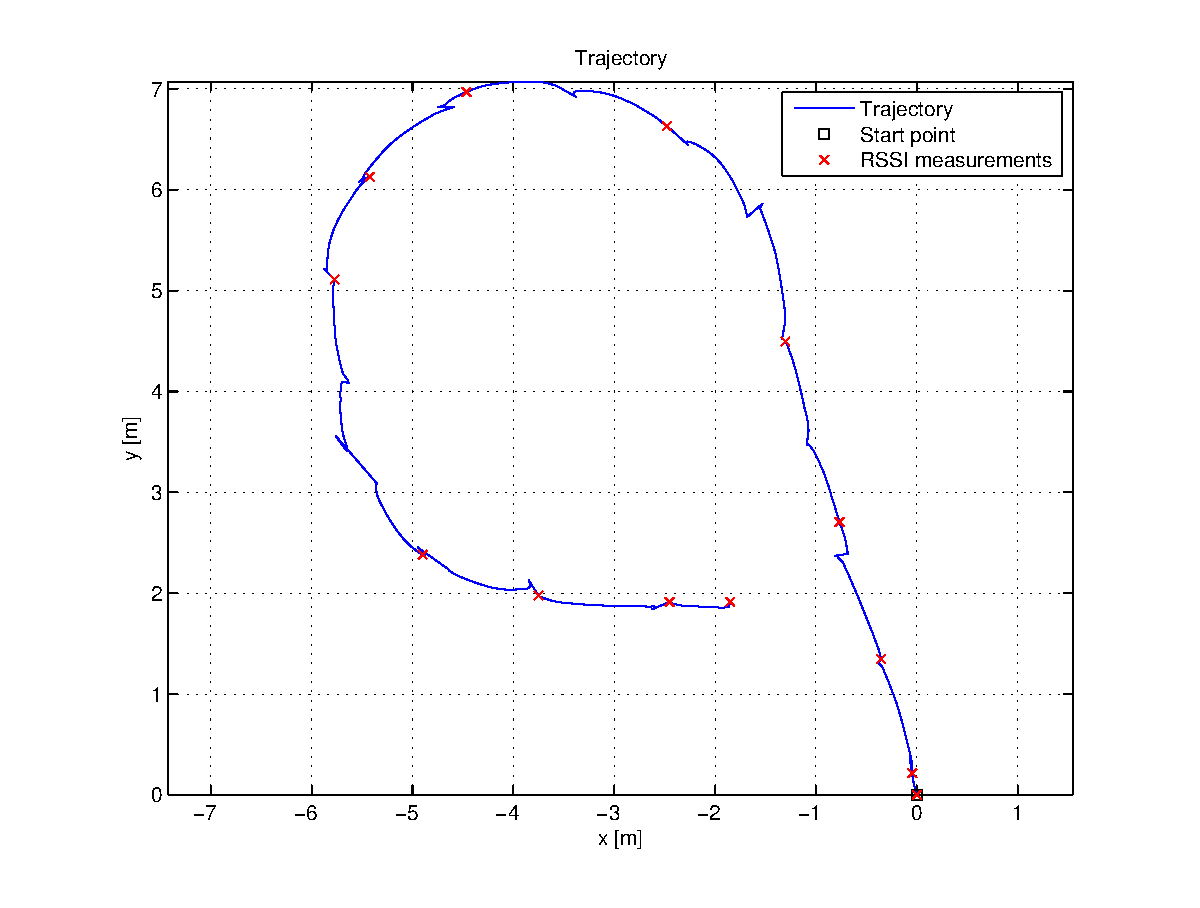
\epsfig{file=path_ex.eps, height=2in, width=2.6in}
% 	\caption{Comparison between point-type and trace-type fingerprinting.}
% 	\label{example1}
% \end{figure}

%\subsection{Key challenges}
%There are some key challenges in training and using the trace-type radio map.
%%\subsubsection{How to model the routes efficiently} This is addressed by an interactive RSS trace calibration method in Section \ref{sec:training}.    
%\subsubsection{How to efficiently generate CTD while avoiding enumerating all routes?} There could be many route combinations in the target area. A generate algorithm based on trace-graph is proposed in Section \ref{sec:training} to generate CTD efficiently.   
%\subsubsection{How to deal with the motion dynamics} People may occasionally slow down, speed up or halt. The walking pattern on the same route can differ greatly in online and offline phases, so measured RSS traces may differ greatly from trained RSS traces. To tolerate such difference, a subsequence dynamic time wrapping algorithm is proposed  for accurate locating, which will be detailed in Section \ref{sec:locating}.  





%
%Note that there could be many different routes. Collecting RSS fingerprints on all these routes one by one can still be very laborious. We propose a measuring, segmentation and graph representation framework for the offline phase. The radio map is stored as a graph, which is easily trained and can generate fingerprints of all route combinations in the online phase. This greatly saves the training efforts.

%Next we discuss the realization techniques in the training phase, including (i) how to simultaneously collect RSSs and positions along a route (Section \ref{data-collect}), and (ii) how to store sequential data in the radio map in an efficient way (Section \ref{radiomap-graph}).

\section{Trace-graph Construction}\label{sec:training}
The input of training problem include: 1) an area of interest (AOI), denoted by $\mathcal{A}$ with its floorplan; 2) a set of APs in the AOI without requiring their locations or total number.  %The output of training process is a graph $G = (V, E)$, which represents the RSS traces of the route segments in the AOI. $V$ stores the cross points of the routes. $E$ stores the RSS traces of the route segments separated by the cross points.  
The training phase is separated into three steps: 1) \emph{trace calibration}; 2) \emph{trace-graph generation} ; 3) \emph{CTB generation}.    

\subsection{Interactive RSS trace calibration} \label{data-collect}
By using smart phones, RSS trace calibration can be easily carried out, which is implemented by developing a trace calibration App. It performs three tasks: 1) rendering the floorplan, 2) defining routes by clicking on the floorplan shown on the screen, and 3) recording the RSS sequences as user moves along the defined routes.   

More specifically, the App loads the floorplan and sets the scaling factor specified by the floorplan so that each pixel on the rendered map are mapped to a location in the AOI. Then for each route to calibrate,  the user clicks on the map to mark the route. One route is often obtained by connecting several clicked points on the screen. Then the user walks along the specified routes to collect a RSS sequence. Since the WiFi-scanner in the App takes RSS samples in equal intervals, the concrete positions where RSSs are measured on the route can be calculated accordingly, assuming that the user is moving at constant speed on each designed segment. A trained RSS trace on a route will be a series of $\langle \text{location}, \text{RSS-vector} \rangle$ pairs. For a trained trace, let $T_i$ be its trajectory and $Y^{(i)}$ be the corresponding RSS sequence. Note that the length of different traces maybe different and the vector length in each pair maybe different for WiFi coverage dynamics. We suppose that there are $n$ trained traces. 
Snapshots of the route and RSS trace calibration App are shown in Fig. \ref{collectApp}. 

%To label the location ground truth in the training phase, we employ intertial navigation system (INS), such as OpenShoe \cite{openshoe}, which enables us to accurately track the position of a walking person. When a person walks with an INS device mounted on his foot, INS can calculate an estimate of his trajectory with a high accuracy.
%Based on INS, the sequential RSS and position data are collected in the offline phase as follows. A person walks through a predetermined route $\Gamma$ with INS mounted on his foot. The INS calculates an estimate of his track during his walk (i.e., outputs, in high frequency, current positions). We approximate the real trajectory $\Gamma$ by the output of INS. In the meantime, we let the same device keep collecting RSSs from wireless access points in the surrounding WiFi network. The positions where RSSs are measured are also recorded.

%If $m$ RSS vectors $y_1, \cdots, y_m$ are sequentially collected during the walk, then for each measurement $y_j$, the position where it is measured is also recorded.

%We implement the above data collection method using OpenShoe. In Fig. \ref{path-example}, we plot the trajectory estimated by OpenShoe during a short walk. The RSSs are collected along this route, and the positions with RSS measurements are highlighted.

\begin{figure}
\centering
\includegraphics[scale=0.8]{collect.pdf}
\caption{Snapshot of trace calibration and RSS collection App}
\label{collectApp}
\end{figure}

\subsection{Construct trace-graph} %
%\color{red}
%We have seen how to collect RSSs and positions along a route.
%Then one way to build the radio map is to measure RSSs along many routes and to store all of them. Ideally, these routes can cover all possible routes in the given rigion.
%However, it is sometimes infeasible or inadvisable to measure and store all possible routes separately due to the following reasons:
%(i) There may be too many possible routes. It costs too much labor, time and memory to measure all of them.
%(ii) There may be many common segments among possible routes. If all routes are measured separately, those common parts will be measured multiple times, which is a waste of time and memory.
%
%Now we introduce a radio map structure based on graph. The motivation is that we can connect several routes together to form a new route. To achieve this, we store the radio map as a graph $G=(V, E)$. Each node $v\in V$ is a position, and each edge $e = (u, v) \in E$ corresponds to a measured segment between $u$ and $v$ (including trajectory and RSS sequence). As a common notion in graph theory, a \emph{path} $P$ in $G$ is a list of edges $(v_1, v_2), (v_2, v_3), \cdots, (v_{k-1},  v_k)$ in $E$. We usually simply represent $P$ as $P = v_1 \text{-} v_2 \text{-} \cdots \text{-} v_k$.
%Then any path $P = v_1 \text{-} v_2 \text{-} \cdots \text{-} v_k$ in $G$ can be regarded as a potential route $\Gamma$ by connecting the segments $(v_1, v_2), \cdots, (v_{k-1}, v_k)$ sequentially. Therefore, we can combine the data collected at edges $(v_1, v_2), \cdots, (v_{k-1}, v_k)$ to obtain the trajectory and the RSS sequence along $\Gamma$.
%
%In principle, by storing the radio map as a graph $G$, every path in $G$ will give a possible route in the given region. Although there could be many paths in $G$ in general, for our purpose it suffices to consider a small number of them.
%%There are, however, infinitely many walks in $G$ (as long as at least one edge exists) -- it is infeasible to consider all of them as candidates. Nevertheless, in most cases it suffices to consider only a finite number of possible walks.
%Since in the online phase people would want to know their location quickly (i.e., in a real-time manner), it makes sense to assume that the route to be located in the online phase is not very long. Thus we can, for example, only consider paths which consist of at most $c$ edges, where $c$ is a certain constant (e.g. $c=2$). Even if the route to be located is very long, we can break it into short pieces and locate these pieces separately.\\
By simplify RSS trace collection along long routes, in next step, we want to generate RSS traces for all the possible routes. 
As shown in Fig. \ref{example2}, suppose we have trained the four routes, the problem is how to generate RSS traces for other possible routes. 
Training them one-by-one is still laborious, because there maybe many combinatorial routes in the AOI. But note that, some of the routes have common parts, so it is not necessary to train these routes separately.
We propose a graph representation for the RSS traces on the indoor routes, which provides an efficient and flexible way to generate the possible candidate routes. 

\subsubsection*{Automatic graph construction}

\begin{figure}[t]
\centering
\includegraphics[scale=0.7]{graph.pdf}
%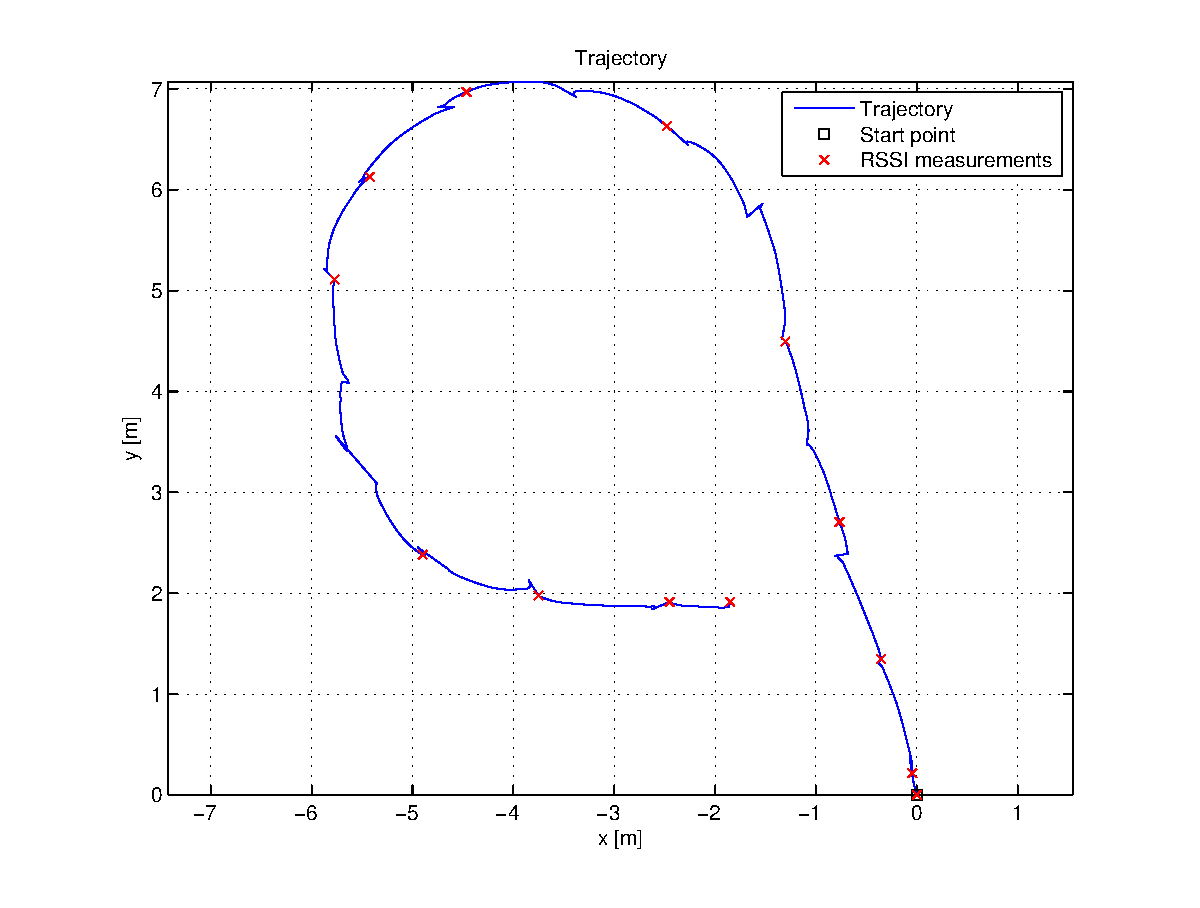
\epsfig{file=path_ex.eps, height=2in, width=2.6in}
\caption{Construct trace graph from calibrated traces.}
\label{example2}
\end{figure}

The basic idea is to construct a graph $G=(V, E)$ from the calibrated traces. The construction is composed of a segmentation step and a connection step. 
In segmentation, if two routes intersect at a common point $v$, $v$ will be recognized and added as a vertex to the graph. Since the trajectories of all calibrated routes are known, we can find all the intersections formed by these routes. The graph vertex set $V$ include the intersection points and the terminal points (i.e., starting and ending points) of all calibrated routes. Then each route is broken into edges by the vertices on it; these edges form the edge set $E$. %Such edges are called \emph{elementary edges}.
%The number of edges is denoted by $N$. 
The graph $G$ is called a \emph{trace-graph}. An example of how a trace-graph is formed by the calibrated traces is shown in Fig. \ref{example2}. 

\subsection{Generate CTD}
\label{radiomap-graph}

%\subsubsection{$c$-edge RSS-trace generation}
Based on the trace-graph, candidate trace database, which worked as online reference for trace matching is generated. Note that the input sequence in the online phase is a short RSS sequence within a given time window, so the offline generated candidate routes do not need to be long, as long as they are confidentially longer than the size of the moving window. This can greatly reduce the route generation and storage complexity.
Hence, we will generate routes by enumerating all paths in $G$ of lengths no more than $c$, i.e., paths that contain at most $c$ edges.
In our implementation, we use $c=3$ or $4$. The route generation algorithm is summarized in Algorithm \ref{alg:route-gen}. Here $\mathcal{P}_k$ contains all paths of length $k$. Let $\mathcal{P}_{k}(i)$ be the $i$th path in $\mathcal{P}_k$, and $E = \{e_1, e_2, \cdots, e_{|E|}\}$.
Note that if a path is generated by Algorithm \ref{alg:route-gen}, its subpaths will not be included.

\begin{algorithm}[h]
\caption{$c$-edge RSS-trace generation}
\label{alg:route-gen}
\begin{algorithmic}
\REQUIRE  $G=(V, E), c$
\ENSURE  Paths containing at most $c$ edges: $\mathcal{P}$
\STATE Add all edges in $E$ to $\mathcal{P}_1$
\FOR {$k=1$ \TO $c-1$}
\FOR {$i=1$ \TO $|\mathcal{P}_k|$}
\FOR {$j=1$ \TO $|E|$}
\IF {$\mathcal{P}_{k}(i)$ and $e_j$ have a common terminal point and $e_j$ is not part of $\mathcal{P}_{k}(i)$}
\STATE Connect $\mathcal{P}_{k}(i)$ and $e_j$, and add the connected route to $\mathcal{P}_{k+1}$ %if there is not the same route
\STATE Mark $\mathcal{P}_{k}(i)$ as ``used"
\ENDIF
\ENDFOR
\ENDFOR
\STATE Delete all ``used" paths from $\mathcal{P}_{k}$
\ENDFOR
\STATE Output $\mathbf{\mathcal{P}}=\mathcal{P}_1 \cup \cdots \cup \mathcal{P}_c$
\end{algorithmic}
\end{algorithm} 

Note that the result CTD contains a set of moderate-size RSS traces, labeled by the routes where they are collected, in the form of $\{(\Gamma_i, Y^{(i)}): i=1,\cdots, L\}$, where $L$ is the total number of traces.  


%For example, suppose that along a route $\Gamma$ there are nodes $v_0, v_1, v_2, \cdots, v_k$, where $v_0$ and $v_k$ are the terminal points of $\Gamma$, and other $v_i$'s ($1\le i\le k-1$) are the intersections between $\Gamma$ and other routes. Then $(v_0, v_1), (v_1, v_2), \cdots, (v_{k-1}, v_k)$ are edges in the graph.
%In this way, we only need to measure some arbitrary routes in the offline phase, and the graph can be constructed automatically by identifying the intersections and segmenting the routes.


%An example is shown in Fig. \ref{radiomap}, where 6 blue routes are measured in the offline phase. The 12 terminal points of these routes, together with the 7 intersections produced by them, will be recognized as the nodes in the graph.

%\color{black}
\begin{theorem}[computational complexity] \emph{
		The time complexity of Algorithm \ref{alg:route-gen} is at most $O(N^{c})$, where $N = |E|$ is the number of edges and $c$ is a small constant.}
\end{theorem}
\begin{proof}
	We always have $|\mathcal{P}_k| \le N^k$ throughout the algorithm. Note that it takes $O(1)$ time to add a new path to the database since $c$ is a constant. Therefore the time used by Algorithm \ref{alg:route-gen} is at most
	$O(\sum_{k=1}^{c-1}  N^{k} \cdot N  ) = O \left( \frac{N^2(N^{c-1}-1)}{N-1} \right) = O(N^{c})$.\\
\end{proof}

\begin{theorem}[size of route database]\emph{
		The number of offline generated routes, i.e., $|\mathcal P|$, is at most $O(N^c)$, where $N = |E|$ is the number of edges. }
\end{theorem}
\begin{proof}
	Since $|\mathcal{P}_k| \le N^k$, the number of routes is at most
	$\sum_{k=1}^c N^k = \frac{N(N^{c} - 1)}{N-1} = O(N^c)$.\\
\end{proof}


\textbf{Remark.} As will be shown in our experiments, the moving window in the online phase is generally required to contain RSS readings when moving for 5-10 meters in order to achieve good accuracy. In most buildings, 10 meters can definitely cover 1 to $4$ route edges, so choosing $c=4$ in our experiments is a good balance between locating accuracy and computational complexity. Further, the offline training phase needs only to be run once, so it is acceptable even if $c$ is large.     


\section{Trace-Type Fingerprinting: Locating Phase} \label{sec:locating}



In this section we present the locating method in trace-type fingerprinting. The basic idea is that RSS is online measured by user's device as the user is moving, which feeds into a moving window containing the latest $n$ measurements of the RSS vectors, denoted by $X = (x_1, \cdots, x_w)$. Note that $x_w$ indicates the current RSS measurement. Then $X$ is searched in the offline trained CTD. The a segment of trace in CTD that best matches with $X$ is detected as the matched subsequence, and the end point of the subsequence is detected as the current position of the user.  
The key challenge is that the moving speed of a user in online phase may differ greatly than that in offline phase. We propose a subsequence dynamic time wrapping (SDTW) algorithm to measure similarity between two temporal sequences that can tolerate the  variances in time or speed.  


\subsection{Dynamic time warping} \label{sec:dtw}
SDTW is an extension of Dynamic Time Wrapping (DTW) \cite{DTW, dtw78}. We briefly review DTW at first. For convenience, we use $[n]$ to represent the set $\{1,2,\cdots,n\}$ for a positive integer $n$. 

\subsubsection*{Classical DTW}
Consider two sequences $X = (x_1, \cdots, x_n)$ and $Y = (y_1, \cdots, y_m)$ whose elements $x_i, y_j (i\in[n], j\in[m])$ are all in the same metric space $\mathcal X$ with a distance function $d: \mathcal X \times \mathcal X \to \mathbb R_{\ge0}$. Let $P = (p_1, \cdots, p_l)$ be an \emph{alignment} between $X$ and $Y$, where $p_k = (i_k, j_k) \in [n] \times [m]$ for each $k\in[l]$. We say that $P$ is a \textit{warping path} if it satisfies the following conditions.
\begin{itemize}
\item Boundary condition:
\begin{equation}
p_1 = (1, 1), p_l = (n, m).
\end{equation}
\item Step size condition:
\begin{equation} \label{step-size}
p_{k+1} - p_k \in \{(0, 1), (1, 0), (1, 1)\} \quad \forall k\in[l-1].
\end{equation}
\end{itemize}

The distance between $X$ and $Y$ given the warping path $P$ is defined as
\begin{equation}
d_P(X, Y) = \sum_{k=1}^l d(x_{i_k}, y_{j_k}).
\end{equation}
A warping path $P^*$ between $X$ and $Y$ is optimal if it achieves the minimum distance among all possible warping paths. This minimum distance is called the \textit{DTW distance} between $X$ and $Y$, denoted by
\begin{equation}
\text{DTW}(X, Y) = \min \{d_P(X, Y): \text{$P$ is a warping path}\}.
\end{equation}

To find an optimal warping path, there is a simple dynamic programming algorithm. Consider the following procedure:
\begin{equation} \label{dtw-initial}
\begin{aligned}
D(i, 1) &= \sum_{i'=1}^i d(x_{i'}, y_1), \quad i\in[n]\\
D(1, j) &= \sum_{j'=1}^j d(x_1, y_{j'}), \quad j\in[m]
\end{aligned}
\end{equation}
%$D(i, 1) = \sum_{i'=1}^i d(x_{i'}, y_1)$ for $i\in[n]$, $D(1, j) = \sum_{j'=1}^j d(x_1, y_{j'})$ for $j\in[m]$, 
\begin{equation} \label{dtw-recursion}
\begin{aligned}
D(i, j) =& \min\{ D(i-1, j-1), D(i-1, j), D(i, j-1) \} \\
&+ d(x_i, y_j), \quad 1<i\le n, 1<j\le m.
\end{aligned}
\end{equation}
It is easy to see that $D(i, j)$ stores the DTW distance between $X_{[1, i]} = (x_1, \cdots, x_i)$ and $Y_{[1, j]} = (y_1, \cdots, y_j)$. Thus we have $\text{DTW}(X, Y) = D(n, m)$. The optimal warping path can be found by tracing all the iterations. The time complexity of this dynamic programming algorithm is $O(mn)$ \cite{DTW}.
\\

%\subsubsection*{Variations} \label{dtw-generalization}
%The classical DTW can be generalized in several ways in order to speed up computations or to better control the waring paths. Here we mention two kinds of generalizations.

%\subsubsection{Step size condition}
%Instead of \eqref{step-size}, we can allow a different step size condition. For instance, we can replace \eqref{step-size} by $p_{k+1} - p_k \in \{(1, 2), (2, 1)\}$. Then, in the dynamic programming algorithm for finding the optimal warping path, we should change the recursion \eqref{dtw-recursion} to $D(i, j) = \min\{ D(i-1, j-2), D(i-2, j-1)\} + d(x_i, y_j)$ and modify initial values \eqref{dtw-initial} accordingly.

%\subsubsection{Local weights}
%If we prefer one or more value(s) for $p_{k+1}-p_k$ among the three possibilities in \eqref{step-size}, we can introduce a weight vector $(w_d, w_h, w_v) \in \mathbb R_{\ge0}^3$ and use the recursion
%\begin{eqnarray}
%D(i, j) = \min\{  D(i-1, j) + w_h \cdot d(x_i, y_j),\nonumber\\
%D(i-1, j-1) + w_d \cdot d(x_i, y_j),\nonumber\\
%D(i, j-1) + w_v \cdot d(x_i, y_j) \}.
%\end{eqnarray}

%We can also combine the above two generalizations, i.e., to introduce local weights for step size conditions different from \eqref{step-size}.\\



\subsubsection*{Subsequence DTW (SDTW)}

In this problem, the online measured RSS sequence $X$ is generally much shorter than the offline trained RSS traces. Let  $Y = (y_1, \cdots, y_m)$ ($n\ll m$) be one of the offline trained RSS traces. Instead of matching $X$ with whole sequence $Y$, the goal is to find a subsequence $Y_{[a, b]} = (y_a, y_{a+1}, \cdots, y_b)$ ($1\le a \le b \le m$) of $Y$ that can best match with $X$, such that
\begin{equation} \label{sub-dtw}
(a^*, b^*) = \underset{(a, b): 1\le a \le b \le m}{\arg \min} \text{DTW}(X, Y_{[a, b]}).
\end{equation}

The solution to \eqref{sub-dtw} can also be found using dynamic programming. In fact, it suffices to change the initial values \eqref{dtw-initial} to
%The details are given in \cite{DTW}.
\begin{equation} \label{sdtw-initial}
\begin{aligned}
D(i, 1) &= \sum_{i'=1}^i d(x_{i'}, y_1), \quad i\in[n]\\
D(1, j) &=  d(x_1, y_{j'}), \quad j\in[m].
\end{aligned}
\end{equation}
Then the same recursion \eqref{dtw-recursion} is used. The index $b^*$ can be found by
\begin{equation} \label{sdtw-find-b*}
b^* = \underset{b\in[m]}{\arg\min} D(n, b),
\end{equation}
and then the index $a^*$ can be determined by tracing the iterations. The computational complexity of this algorithm is also $O(mn)$.

%The solution to \eqref{sub-dtw} can also be found using dynamic programming. Since we no longer require $x_1$ to be aligned with $y_1$, we can modify the initial values to $D(i, 1) = \sum_{i'=1}^i d(x_{i'}, y_1), D(1, j) = d(x_1, y_j)$ and compute $D(i, j)$ for all $i\in[n], j\in[m]$ using \eqref{dtw-recursion}. Then the optimal ending position $b^*$ can be determined by
%\begin{equation}
%b^* = \underset{b: 1\le b\le m}{\arg \min} D(n, b).
%\end{equation}

%After finding $b^*$, the value of $a^*$ and the optimal warping path can be determined from the optimal warping path $P = (p_1, \cdots, p_l)$ between $X$ and $Y_{[1, b^*]}$ (which is found by the dynamic programming algorithm). Given path $P$, $a^*$ is the largest index such that $p_t = (1, a^*)$ for some $t\in[l]$, and $P' = (p_t, \cdots, p_l)$ is the optimal warping path between $X$ and $Y_{[a^*, b^*]}$.

%Similarly, the generalizations discussed in Section \ref{dtw-generalization} can be incorporated in SDTW.

\subsection{Locating by SDTW} \label{locate-dtw}

As introduced in Section \ref{radiomap-graph}, after the offline training phase, a candidate trace database is constructed, which generates a set of $L$ candidate routes, denoted as $\Gamma^{(1)}, \cdots, \Gamma^{(L)}$. For a route $s\in[L]$, let $Y^{(s)} = (y^{(s)}_1, \cdots, y^{(s)}_{m_s})$ be the sequence of RSS vectors along the route $\Gamma^{(s)}$. 

In the online phase, a person walks along a route $\Gamma'$ while measuring RSSs. Let $X = (x_1, \cdots, x_w)$ be the RSS vector measured in the moving window, then online matching is to align $X$ to a subsequence of some $Y^{(s)}$, i.e., $Y^{(s)}_{[a, b]}$ of $Y^{(s)}$. The current location of the target will then be given as $Y^{(s)}_b$. 

A distance function on the space of RSS vectors is defined as the $l_2$-norm of the RSS vector:
\begin{equation}
d(X, Y) = \| X-Y \|_2 %= \sqrt{\sum_{i=1}^{D}(r_{x,i}-r_{y,i})^2}
\end{equation}
where $X$ and $Y$ are the RSS vectors with the same dimension. A preprocessing is used  when the measured RSS vector and the trained RSS have different lengths; details are given in Section \ref{sec:eval}. 

 
%After specifying a distance function on the space of RSS vectors (e.g. $\ell_p$-norm $d(x, y) = \| x-y \|_p$ in $\mathbb R^d$ for some $p>0$), we can apply SDTW algorithm to find the optimal alignment between $X$ and any subsequence of $Y^{(s)}$. DTW is suitable for dealing with time deformations and different speeds in time series, which makes it a natural fit for our problem since people may walk with different or varying speeds.

Since we do not know in advance which route $\Gamma^{(s)}$ is the one $\Gamma'$ belongs to, we need to find $s^*\in[L]$ such that $X$ can be optimally matched to a subsequence of $Y^{(s^*)}$. Therefore we want to find
\begin{equation}\label{multi-path-opt}
(s^*, a^*, b^*) = \underset{(s, a, b): s\in[L], 1\le a \le b \le m_s}{\arg\min} \text{DTW}(X, Y^{(s)}_{[a, b]}).
\end{equation}

To solve \eqref{multi-path-opt}, we use SDTW to find for every $s\in[L]$ the optimal alignment between $X$ and a subsequence of $Y^{(s)}$, and choose $s^*$ as the one that achieves the minimum DTW distance. Then the location of $Y_{b^*}^{(s^*)}$ is recognized as the current location of the target. 
For each $s\in[L]$, finding the optimal alignment between $X$ and a subsequence of $Y^{(s)}$ by SDTW requires $O(w\cdot m_s)$ time. Therefore the total time used for solving \eqref{multi-path-opt} is $O(w\sum_{s=1}^L m_s) = O(wL\max_{s\in[L]}m_s)$. Combining this with Theorem 2, we have the following theorem.

\begin{theorem} \emph{
	Suppose that the number of RSS measurements in the online phase is $w$. Then the time complexity of online locating by SDTW is $O(c_0w|E|^c)$}, where $c_0$ is the maximum number of RSS measurements in any $c$-edge route in $G = (V, E)$.
	\end{theorem}
\begin{proof}	
	By Theorem~2, The total number of RSS measurements in CTD is at most $c_0 \cdot |E|^c$. Then the time complexity of using SDTW to determine the current location is bounded by $O(c_0w|E|^c)$.
\end{proof}



%
%\begin{figure}
%	\centering
%	\includegraphics[scale=0.3]{B_one_single_trace.pdf}
%	%\epsfig{file=CDF.eps, height=1.8in, width=2.1in}
%	\caption{Floorplan of experiment environment.}
%	\label{env}
%\end{figure}

 \begin{figure*}[htbp]
 	\centering
 	\begin{minipage}[t]{0.33\linewidth}
 		\centering
 		\includegraphics[width=2.3in]{len3-2.png}
 		\caption{CDF of locating error when $w=3$}
 		\label{fig:side:a}
 	\end{minipage}%
 	\begin{minipage}[t]{0.33\linewidth}
 		\centering
 		\includegraphics[width=2.3in]{len5-2.png}
 		\caption{CDF of locating error when $w=5$}
 		\label{fig:side:b}
 	\end{minipage}%
 	\begin{minipage}[t]{0.33\linewidth}
 		\centering
 		\includegraphics[width=2.3in]{len10-2.png}
 		\caption{CDF of locating error when $w=10$}
 		\label{fig:side:c}
 	\end{minipage}
 	\begin{minipage}[t]{0.33\linewidth}
 		\centering
 		\includegraphics[width=2.3in]{len15-2.png}
 		\caption{CDF of locating error when $w=15$}
 		\label{fig:side:d}
 	\end{minipage}%
 	\begin{minipage}[t]{0.33\linewidth}
 		\centering
 		\includegraphics[width=2.3in]{len20-2.png}
 		\caption{CDF of locating error when $w=20$}
 		\label{fig:side:e}
 	\end{minipage}%
 \end{figure*}


 \section{Implementation and Performance Evaluation} \label{sec:eval}
 \subsection{Implementation}
 We develop the trace-type fingerprinting framework using Android platform and the location server is developed by Matlab 2014. The android App carries out the functions including route calibration, RSS traces collection, data transmission to server, and location rendering in the online phase. The server based on Matlab is responsible for conducting trace-map construction and the online localization. 
 
 \subsubsection{Data preprocessing} 
 In  trace-type fingerprinting implementation, the collected RSS sequence information has to be preprocessed, because the number and order of detected APs at different locations are rather different. In the preprocessing step, we represent the measured RSS vectors in the same length and rearrange the RSS values in each vector so that each coordinate corresponds to a fixed AP.
 
 
 In particular, the distinct MAC addresses of APs are counted to form a AP vector. Then,  every measured RSS vector is projected to a vector having the same length of the AP vector. Since RSS from some APs cannot be detected at certain locations, a constant is filled as the RSS of the out-of-the-range AP. We test how the filled constant value affects the locating performances, which is presented in Section \ref{eval_fill}. 
 
 
 
 
 
 
 %\begin{figure}[t]
 %\centering
 %\includegraphics[scale=0.6]{collect.pdf}
 %%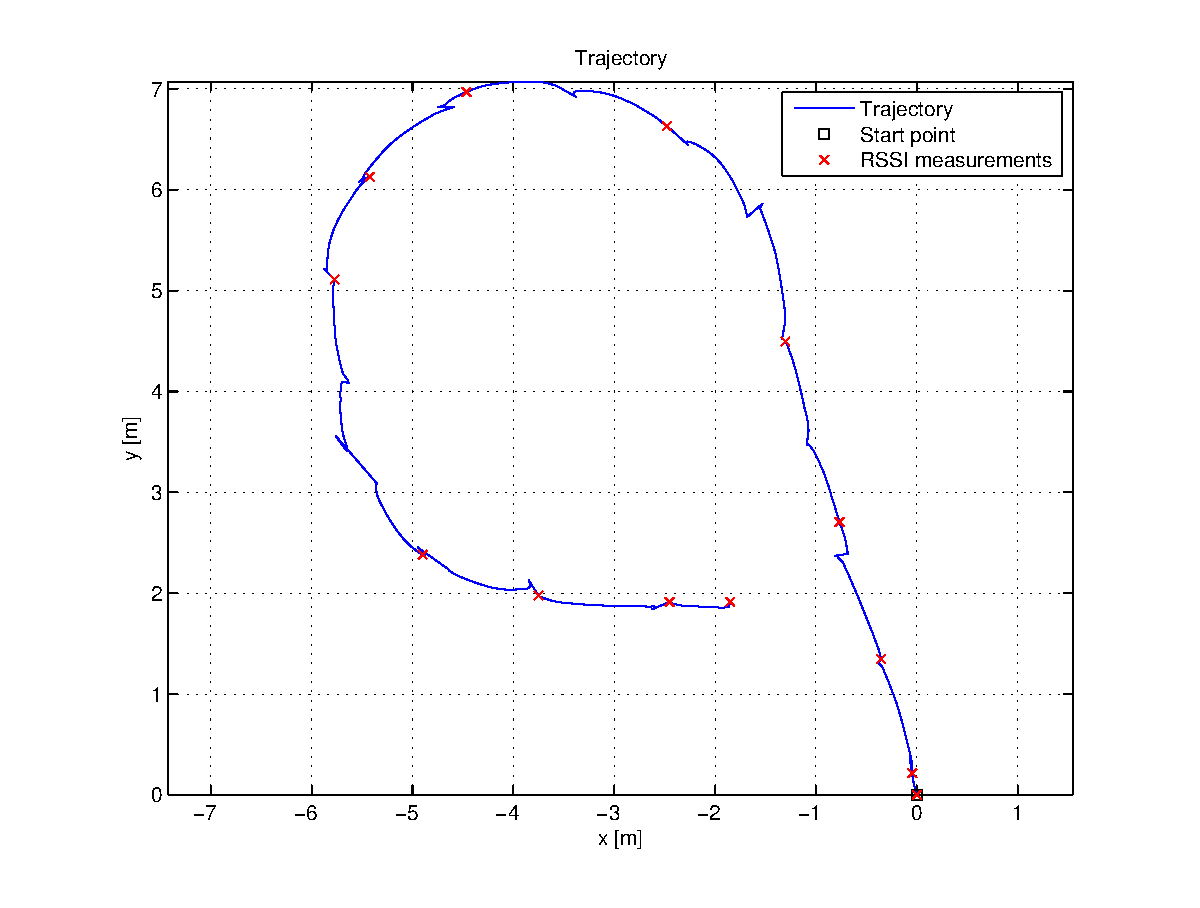
\epsfig{file=path_ex.eps, height=2in, width=2.6in}
 %\caption{Snapshots of Wiloc App}
 %\label{snapshot}
 %\end{figure}
 %We perform simulation tests to evaluate the localization accuracy of sequence-type location fingerprinting.
 %The simulation is conducted in \textsc{Matlab} environment. We use the floorplan of the 3rd floor of Meng Mingwei Science and Technology Building (South) at Tsinghua University, which has size $17\times60\text{m}^2$. We randomly generate 20 positions in the area for access points, and we use the radio signal propogation model \cite{RSS, Martin10, RSS2} to calculate RSSs at any position based on its distance to the access points.
 %Fig. \ref{radiomap} shows the floorplan with 20 randomly generated positions of access points.
 %
 %%\begin{figure}
 %%\centering
 %%\includegraphics[scale=0.3]{path-ex.pdf}
 %%\epsfig{file=APs.eps, height=1.3in, width=3.7in}
 %%\caption{The floorplan used in the simulation. Blue squares represent the positions of access points.}
 %%\label{map-and-ap}
 %%\end{figure}
 %
 %We simulate the human walking process by clicking on the floorplan. Each route is obtained by connecting the clicked positions by line segments. On each route, RSS vectors are measured about every 0.6m. In the offline phase, we specify several routes to measure and then use the segmentation method (in Section \ref{radiomap-graph}) to construct the radio map as a graph.
 %Fig. \ref{radiomap} shows an example where 6 routes are measured in the offline phase.
 %
 %\begin{figure}
 %\centering
 %%\includegraphics[scale=0.3]{path-ex.pdf}
 %\epsfig{file=radiomap.eps, height=1.3in, width=3.7in}
 %\caption{The floorplan used in the simulation. Red squares stand for the positions of access points. The 6 blue routes are measured in the offline phase. They produce 7 intersections, and the radio map will be a graph of 19 nodes.}
 %\label{radiomap}
 %\end{figure}
 %
 %In the online phase, we also use mouse clicks to specify a route to be located. Recall that we need to take a set of paths in the graph as candidate routes. In our setting, we consider all the paths which start and end at terminal nodes and contain at most one intersection. In other words, a path that we take is either a measured route from the offline phase or start from one route and turn to another route at their intersection.
 %Then, for the route given in the online phase, SDTW (using $\ell_2$ norm as distance measure) is used to determine its location.
 %To evaluate the locating accuracy of our method, we also implement $k$ nearest neighbors (KNN)\footnote{Given an RSS vector, KNN finds $k$ closest RSS vectors in the database, and outputs the average of the $k$ corresponding locations.} algorithm \cite{learning_locate} to determine the location, which is widely-used in point-type location fingerprinting. Fig. \ref{locating} shows two examples of localization results. As we observe from a large number of results (including Fig. \ref{locating}), KNN tends to be very unstable, and SDTW usually finds an accurate estimated location. The results illustrate the robustness of sequence-type fingerprinting method over point-type method.
 %
 %\begin{figure}
 %\centering
 %%\includegraphics[scale=0.3]{path-ex.pdf}
 %\epsfig{file=locate_ex1.eps, height=1.3in, width=3.5in}
 %\epsfig{file=locate_ex2.eps, height=1.3in, width=3.5in}
 %\caption{Locating results given by SDTW and KNN ($k=3$). The radio map is the same as Fig. \ref{radiomap}. The green routes are the ones that we want to locate; the magenta routes are the locating results given by SDTW; the black dashed routes are obtained by connecting locations output by KNN.}
 %\label{locating}
 %\end{figure}
 %
 %We quantitively compare the locating accuracy of SDTW with KNN. We use the radio map given in Fig. \ref{radiomap}, and independently generate 100 random testing routes as follows: (i) randomly select one path from all the candidate paths; (ii) randomly choose a segment from the route corresponding to this path; (iii) on this segment, add a small Gaussian noise to all the fingerprinted positions, and connect these positions to obtain a testing route. For each testing routes, we use SDTW and KNN to estimate its location, and calculate the average locating errors (i.e., the distance between real position and estimated position) over fingerprinted points. The empirical CDFs of locating errors are given in Fig. \ref{CDF}, which shows that SDTW significantly outperforms KNN in terms of locating accuracy. The average locating errors of SDTW, KNN ($k=2$) and KNN ($k=3$) over the testing routes are 0.51m, 1.21m and 1.18m, respectively. The average error of SDTW is less than 44\% of the error of KNN.
 %
 %\begin{figure}
 %\centering
 %%\includegraphics[scale=0.3]{path-ex.pdf}
 %\epsfig{file=CDF.eps, height=1.8in, width=2.1in}
 %\caption{The empirical CDFs of locating errors of SDTW and KNN.}
 %\label{CDF}
 %\end{figure}

 
 \subsubsection{Implementing of the locating phase}
 Locating phase includes collecting the real-time RSS sequences during movement, and finding one optimal matched subsequences of the training set to infer the concrete user location. For data collection, the user just holds the mobile phone and collects real-time sequence of his movement. The latest $w$ RSS vectors forms the moving window. Similar to the training phase, the collected RSS sequences are also preprocessed. We study the impact of the size of the moving window on the locating accuracy. The details are given in Section \ref{eval_acc}. 
 
 
\subsection{Experiment setup}
Experiments are mainly conducted on the third floor of Meng Mingwei Science and Technology (South) Building at Tsinghua Universally, which has size $17\times60 m^2$. %The floorplan of the experiment environment is shown in Fig.  \ref{env}, with several routes plotted on the map. 
In the offline phase, we walk through the corridor and offices to generate the trace-graph and the candidate route database. In the online phase, we take 16 testing traces.%, which are used to test the accuracy and the robustness of the trace-type fingerprinting method.
The results are compared with the traditional $K$-nearest Neighbor (KNN) locating method. In KNN, the online matching is done by finding $K$ most similar RSS vectors from the whole training set and calculating the mean of these $K$ locations as the estimated location of the target.  We mainly evaluate:
\begin{enumerate}
	\item The locating accuracy performance, i.e. how trace-type fingerprinting affects the locating accuracy compared with point-type fingerprinting. 
	\item The locating robustness, i.e. how the changes of environments and devices affect the locating accuracy of trace-type fingerprinting.
\end{enumerate}
 
 
 
 
 
 %For accuracy test we varies the length of moving window, to verify how the locating accuracy is affected by the sequence matching. For robustness test, we conducted training and experiments at different times, to verify the robustness to environment change. We also 
 
 %We used Mi-phone to collect data in the training phase and used Mi-phone, Nexus and Huawei phones in the online phase to test the accuracies of using different devices. We conducted location test at different time to test the locating robust 
 
 \subsection{Accuracy vs. length of moving window}
 \label{eval_acc}
 A key point to evaluate is how trace-type fingerprinting improves the locating accuracy. We evaluate this by varying the length of the moving window and testing how the size of trace affects the locating accuracy.
 
 
 \begin{figure}[htbp]
 	\centering
 	\includegraphics[width=3in]{len.png}
 	\caption{Mean locating error as a function of $w$}
 	\label{fig:side:f}
 \end{figure}
 
 We test the locating accuracy performance by varying the size of moving window as 3, 5, 10, 15, and 20, and evaluating the locating accuracy in each case. In each setting of the moving window size, we independently generate 500 random testing traces from the 16 long testing traces. The generation method is: (i) randomly select one trace from 16 training traces; (ii) randomly choose a length-$w$ window from the chosen trace. For example, when $w=10$, 500 random testing traces, each containing 10 RSS vectors are generated on the 16 long testing traces. We use SDTW and KNN to estimate the end point locations of these 500 traces. The locating error is the Euclidean distance from the ground truth position to the estimated position. 
 
 Fig. \ref{fig:side:a} to Fig. \ref{fig:side:e} show the empirical cumulative distribution functions (CDF) of the locating error when the moving window size varies from 3 to 20. The locating errors of KNN ($k=2$ and $3$) are also plotted for comparison. We can find a general trend that, the longer the moving window is, the better the locating accuracy is. When $w=3$, SDTW is almost degraded to KNN. When $w>5$, SDTW shows remarkable locating accuracy improvement than KNN. In all the experiments with $w \ge 5$, SDTW shows better locating accuracy than KNN. 
 
 The average locating error as a function of the size of moving window $w$ is plotted in Fig. \ref{fig:side:f}. It clearly shows how the moving window size affects the locating error. 
 We  observe that  SDTW provides better accuracy when the moving window size is larger than 5, and that its accuracy sharply outperforms KNN in such settings. When the length is too short, SDTW is almost degraded to KNN. After $w>10$, when the moving window size increases, the locating accuracy tends to decrease a little bit. The reason might be that when $w$ is longer, the accuracy decreases at some boundary locations, because it is hard to form a long sequence. So a window size between $5$ and $10$ is appropriate. 
 Note that when RSS sampling rate is 1 Hz, user moves about 5-10 meters during this period, which is acceptable in real applications. 
 
 
 
 
 %$Fig.B_general_performance$ shows the general performance of two algorithms and we can conclude that TraceGraph works better than KNN. The average locating errors of SDTW, KNN(k=2) and KNN(k=3) are 2.5m, 4.0m, 3.7m, respectively.  
 
 
 \subsection{Locating robustness vs. environment changes}
 
 In this section, we assess the effect of environment changes on the locating accuracy of trace-type fingerprinting.  It is evident that the calibration effort is the major cost of using fingerprinting method. If the trained fingerprint can be robust to environment changes, frequent recalibration will not be needed, which will save the calibration cost. 
 
 
 For testing the impacts of environment changes, we collected one set of training records at 3:00-4:00pm, July 23, 2015 and use it to construct the trace-graph and candidate route database. Then, we collected three sets of testing traces at three different times. Set 1 was collected at 4:00-5:00pm, July 23, 2015. Set 2 was collected at 10:00-11:00am, July 25, 2015. Set 3 was collected at 2:00-3:00pm, July 31, 2015. The temperature when collecting Set 3 is most close to that when collecting the training set.  We use SDTW and KNN to calculate the locating errors of these three sets. We use window size $w=10$ in SDTW in these experiments. The mean locating errors of the three experiments are shown in Fig. \ref{env1}.
 
 We can see that both SDTW and KNN keep reasonable locating accuracy when the test times differ from the training time. One reason may be that the indoor environment was kept almost the same by the air conditioner. But overall, STDW still has much better locating accuracy than KNN. This shows that we need not frequently update CTD.  
 
 
 
 \begin{figure}[htbp]
 	\centering
 	\includegraphics[scale=0.5]{envs.png}
 	%\epsfig{file=CDF.eps, height=1.8in, width=2.1in}
 	\caption{Mean locating errors in three sets of experiments investigating the impacts of environment changes.}
 	\label{env1}
 \end{figure}
 
 \subsection{Locating robustness vs. device changes}
 We also evaluate how the change of locating devices affect the locating accuracy. 
 
 In this experiment,
 we use Mi-phone to collect the training traces and to construct the trace-graph and the candidate route database. Then, we choose three different mobile phones, i.e., Mi-phone, Huawei-Pad and Nexus-phone to conduct online testing. We calculate the locating errors in each group of testing. The empirical CDFs of the locating error are shown in Fig. \ref{dev}. We find that both SDTW and KNN are worse when the training device is different from the online locating device, because different devices may have different sensitivity to the nearby AP signal strengths. This difference  leads to the accuracy performance degradation when changing to a different device in the online phase. 
 
 Nevertheless, we observe that SDTW is still more robust than KNN when the testing device is different from the training device. We can see that some serious errors appear in KNN when the testing devices are changed. For example,  for the Nexus group, about 10\% of locating errors are beyond 10m. Such performance degradation is not acceptable. But SDTW still provides reasonable accuracy, with mean locating error less than 3 meters, which shows its robustness to device changes. 
 
 
 \begin{figure}[t]
 	\centering
 	\includegraphics[scale=0.5]{dev.png}
 	%\epsfig{file=CDF.eps, height=1.8in, width=2.1in}
 	\caption{CDF of locating error when locating device changes.}
 	\label{dev}
 \end{figure}
 
  \subsection{Robustness vs. walking pattern dynamics}
  
  In the training phase, the RSS traces are collected while user moves in almost constant speed, but we cannot expect the users in online phase to walk in constant speed. Users may occasionally halt and then start walking again, or may change their walking speed frequently. 
  
  To evaluate SDTW's tolerance to the walking speed and walking pattern variances, we design a set of experiments. The tester moves in a walk-stop pattern, i.e., walks, stops, and then walks again repeatedly. The collected window of RSS sequences are searched in CTD using STDW to locate the user.
  We compare SDTW with an equal-length matching algorithm in which the subsequence in CTD that has the same length $w$ and the has the shortest distance to the measured trace is detected as the location route. 
  
 
 
 \begin{figure}[htbp]
 	\begin{minipage}[t]{0.5\linewidth}
 		\centering
 		\includegraphics[width=1.7in]{w1.png}
 		\caption{Sequence matching by SDTW}
 		\label{w1}
 	\end{minipage}%
 	\begin{minipage}[t]{0.5\linewidth}
 		\centering
 		\includegraphics[width=1.7in]{w2.png}
 		\caption{Equal-length sequence matching}
 		\label{w2}
 	\end{minipage}%
 \end{figure}
 
 The matching result of one instance is shown in Fig. \ref{w1} and Fig. \ref{w2}. SDTW matches the moving window with indices 10-20 to a subsequence with indices 16-19 in CTD. The stopping sequence was efficiently wrapped. However, equal-length matching cannot wrap the RSSs at the stopping time. The figure shows the adaptivity of SDTW. Furthermore, the empirical CDF of locating error in the series of walk-stop experiments is plotted in Fig. \ref{wait-stop}, which shows that SDTW performs the best. It is interesting to see that equal-length matching is a little better than KNN, which shows the accuracy improvement of trace-type matching over point-to-point matching.
 
 \begin{figure}[t]
 	\centering
 	\includegraphics[scale=0.5]{waits1.png}
 	%\epsfig{file=CDF.eps, height=1.8in, width=2.1in}
 	\caption{CDF of locating error in walk-stop experiment.}
 	\label{wait-stop}
 \end{figure}
 
 \subsection{Robustness vs.  filled RSS value for out-of-the-range APs}
 \label{eval_fill}
 
 As mentioned in the implementation section, in data preprocessing, the RSSs of the out-of-the-range APs are filled by a constant value in order to turn the RSS vectors into equal length. We study the impact of this filled value to the locating accuracy.
 
 We evaluated three cases by setting the filled value to $0$, $-100$ and $-200$. The empirical CDFs of locating errors are plotted in Fig. \ref{filler}.  It shows that the difference of the filling values has little impact on the locating accuracy. The reason is that the out-of-the-range APs in the offline training phase highly consistent with the out-of-the-range APs in the online phase. This shows that the DTW distance is mainly determined by the RSSs of the nearby APs.% and that the filled value is not important for our purpose.
 
 
 
 
 \begin{figure}[htbp]
 	\centering
 	\includegraphics[scale=0.5]{filler.png}
 	%\epsfig{file=CDF.eps, height=1.8in, width=2.1in}
 	\caption{CDF of locating error when filling different values to the RSSs of out-of-the-range APs.}
 	\label{filler}
 \end{figure}
 
 
 \section{Conclusion, Discussion, and Future work}
 \label{sec:conclusion}
 This paper presents design methodologies and performance evaluations of a novel trace-type fingerprint method for indoor locating. It is designed to implicitly model the user movement continuity and indoor path constraint into the trace-type fingerprint, while making the training phase easier and the online matching phase more robust.
 By proposing CTD and STDW, the trace-type fingerprinting method is designed to have low complexity while being very effective. The analysis and performance evaluations show comprehensive merits over the traditional point-type radio map methods. 
 \subsection{Merits}
 \subsubsection{Easier to train} Training can be easily carried out by holding a mobile device and walking along marked routes. The trace-graph generation algorithm is responsible for generating CTD for online reference. This process is much easier than the point-by-point RSS fingerprint calibration. 
 \subsubsection{Better accuracy} Trace-type fingerprinting provides better locating accuracy than point-type fingerprinting. 
 \subsubsection{Better robustness}
 It is more robust under environment changes and device changes. 
 
 \subsection{Limitations}
 A limitation of trace-type fingerprinting method is that it is a little complex to be used in large hall-like areas, because there may be innumerable number of routes. An approach is to calibrate routes in grid topology and generate grid topology trace-graph. Although the complexity to generate candidate routes from the dense grid topology trace-graph is high, because it needs to be run only once, it is still possible to use. Further, it might be possible to combine point-type fingerprinting and trace-type fingerprinting in hall-like areas. In this paper we focus on trace-type fingerprinting and leave the combination work into future. 
 
 \subsection{Future work} 
 There are still many problems to explore in the future. 
 
 1) \emph{How to design hierarchical method to partition large-scale environment?}
 Since each AP has limited coverage area, an idea of hierarchical locating is to firstly narrow down the location space by matching AP lists, and then to conduct sequence matching within the smaller area. We leave this to future work.
 
 2) \emph{Sensor fusion to construct traces of multiple features.} Today's smart phones contain a set of sensors including inertial sensors, compass, light sensors, acoustic sensors, etc. By training trace-type fingerprint containing multi-type sensor features, the locating accuracy and robustness can be further improved by sensor fusion and sequence matching. 
 
 3) \emph{Energy efficiency in online matching is also an important problem.} Since mobile phones have limited battery, how to save energy while using the locating service is an important issue. It can be explored by taking samples more sparsely and integrating with the user moving model. 

%\section{Conclusion and Final Remarks} \label{sec:conclusion}
%
%In this paper we propose a new location fingerprinting method based on sequence. It does not require laborious work in the offline training phase, and is more robust and accurate than tradition point-type fingerprinting. Our method is particularly suitable for places constrained by routes, in which potential locations are almost covered by a set of routes.
%
%In addition to simulation, we have implemented the locating system using the techniques described in this paper. Detailed results and analysis of real experiment will be presented in the full version of the paper.


% An example of a floating figure using the graphicx package.
% Note that \label must occur AFTER (or within) \caption.
% For figures, \caption should occur after the \includegraphics.
% Note that IEEEtran v1.7 and later has special internal code that
% is designed to preserve the operation of \label within \caption
% even when the captionsoff option is in effect. However, because
% of issues like this, it may be the safest practice to put all your
% \label just after \caption rather than within \caption{}.
%
% Reminder: the "draftcls" or "draftclsnofoot", not "draft", class
% option should be used if it is desired that the figures are to be
% displayed while in draft mode.
%
%\begin{figure}[!t]
%\centering
%\includegraphics[width=2.5in]{myfigure}
% where an .eps filename suffix will be assumed under latex, 
% and a .pdf suffix will be assumed for pdflatex; or what has been declared
% via \DeclareGraphicsExtensions.
%\caption{Simulation Results}
%\label{fig_sim}
%\end{figure}

% Note that IEEE typically puts floats only at the top, even when this
% results in a large percentage of a column being occupied by floats.


% An example of a double column floating figure using two subfigures.
% (The subfig.sty package must be loaded for this to work.)
% The subfigure \label commands are set within each subfloat command, the
% \label for the overall figure must come after \caption.
% \hfil must be used as a separator to get equal spacing.
% The subfigure.sty package works much the same way, except \subfigure is
% used instead of \subfloat.
%
%\begin{figure*}[!t]
%\centerline{\subfloat[Case I]\includegraphics[width=2.5in]{subfigcase1}%
%\label{fig_first_case}}
%\hfil
%\subfloat[Case II]{\includegraphics[width=2.5in]{subfigcase2}%
%\label{fig_second_case}}}
%\caption{Simulation results}
%\label{fig_sim}
%\end{figure*}
%
% Note that often IEEE papers with subfigures do not employ subfigure
% captions (using the optional argument to \subfloat), but instead will
% reference/describe all of them (a), (b), etc., within the main caption.


% An example of a floating table. Note that, for IEEE style tables, the 
% \caption command should come BEFORE the table. Table text will default to
% \footnotesize as IEEE normally uses this smaller font for tables.
% The \label must come after \caption as always.
%
%\begin{table}[!t]
%% increase table row spacing, adjust to taste
%\renewcommand{\arraystretch}{1.3}
% if using array.sty, it might be a good idea to tweak the value of
% \extrarowheight as needed to properly center the text within the cells
%\caption{An Example of a Table}
%\label{table_example}
%\centering
%% Some packages, such as MDW tools, offer better commands for making tables
%% than the plain LaTeX2e tabular which is used here.
%\begin{tabular}{|c||c|}
%\hline
%One & Two\\
%\hline
%Three & Four\\
%\hline
%\end{tabular}
%\end{table}


% Note that IEEE does not put floats in the very first column - or typically
% anywhere on the first page for that matter. Also, in-text middle ("here")
% positioning is not used. Most IEEE journals/conferences use top floats
% exclusively. Note that, LaTeX2e, unlike IEEE journals/conferences, places
% footnotes above bottom floats. This can be corrected via the \fnbelowfloat
% command of the stfloats package.








% conference papers do not normally have an appendix


% use section* for acknowledgement
%\section*{Acknowledgment}


%The authors would like to thank...





% trigger a \newpage just before the given reference
% number - used to balance the columns on the last page
% adjust value as needed - may need to be readjusted if
% the document is modified later
%\IEEEtriggeratref{8}
% The "triggered" command can be changed if desired:
%\IEEEtriggercmd{\enlargethispage{-5in}}

% references section

% can use a bibliography generated by BibTeX as a .bbl file
% BibTeX documentation can be easily obtained at:
% http://www.ctan.org/tex-archive/biblio/bibtex/contrib/doc/
% The IEEEtran BibTeX style support page is at:
% http://www.michaelshell.org/tex/ieeetran/bibtex/
%\bibliographystyle{IEEEtran}
% argument is your BibTeX string definitions and bibliography database(s)
%\bibliography{IEEEabrv,../bib/paper}
%
% <OR> manually copy in the resultant .bbl file
% set second argument of \begin to the number of references
% (used to reserve space for the reference number labels box)
%\begin{thebibliography}{1}

%\bibitem{IEEEhowto:kopka}
%H.~Kopka and P.~W. Daly, \emph{A Guide to \LaTeX}, 3rd~ed.\hskip 1em plus
%  0.5em minus 0.4em\relax Harlow, England: Addison-Wesley, 1999.

%\end{thebibliography}

\bibliographystyle{IEEEtran}
\bibliography{sequence_locate_paper}




% that's all folks
\end{document}


